% !TeX spellcheck = en_GB
\section{Thickness, Sea level pressure, moisture, and wind at \SI{250}{\hPa}}
\label{sec:Geop}
A good overview gives the sea level pressure, \SI{1000}-\SI{500}{\hPa} thickness map and winds at \SI{250}{\hPa}. \Cref{fig:GeopJet} shows, that it combines several important features of the vertical distribution within the atmosphere, for example.\\
Black contour lines indicate sea level pressure in \SI{}{\hPa} and makes it possible to observe cyclones and anticyclones at the sea surface. 
%%% Geopot Jet maps %%%%%%%%%%%%%%%%%%%%%%%%%%%%%%%%%%%%%
% !TeX spellcheck = en_GB

\begin{figure}[h!]
    \centering
%%%%%% 20/12
    \begin{subfigure}[b]{0.49\textwidth}
        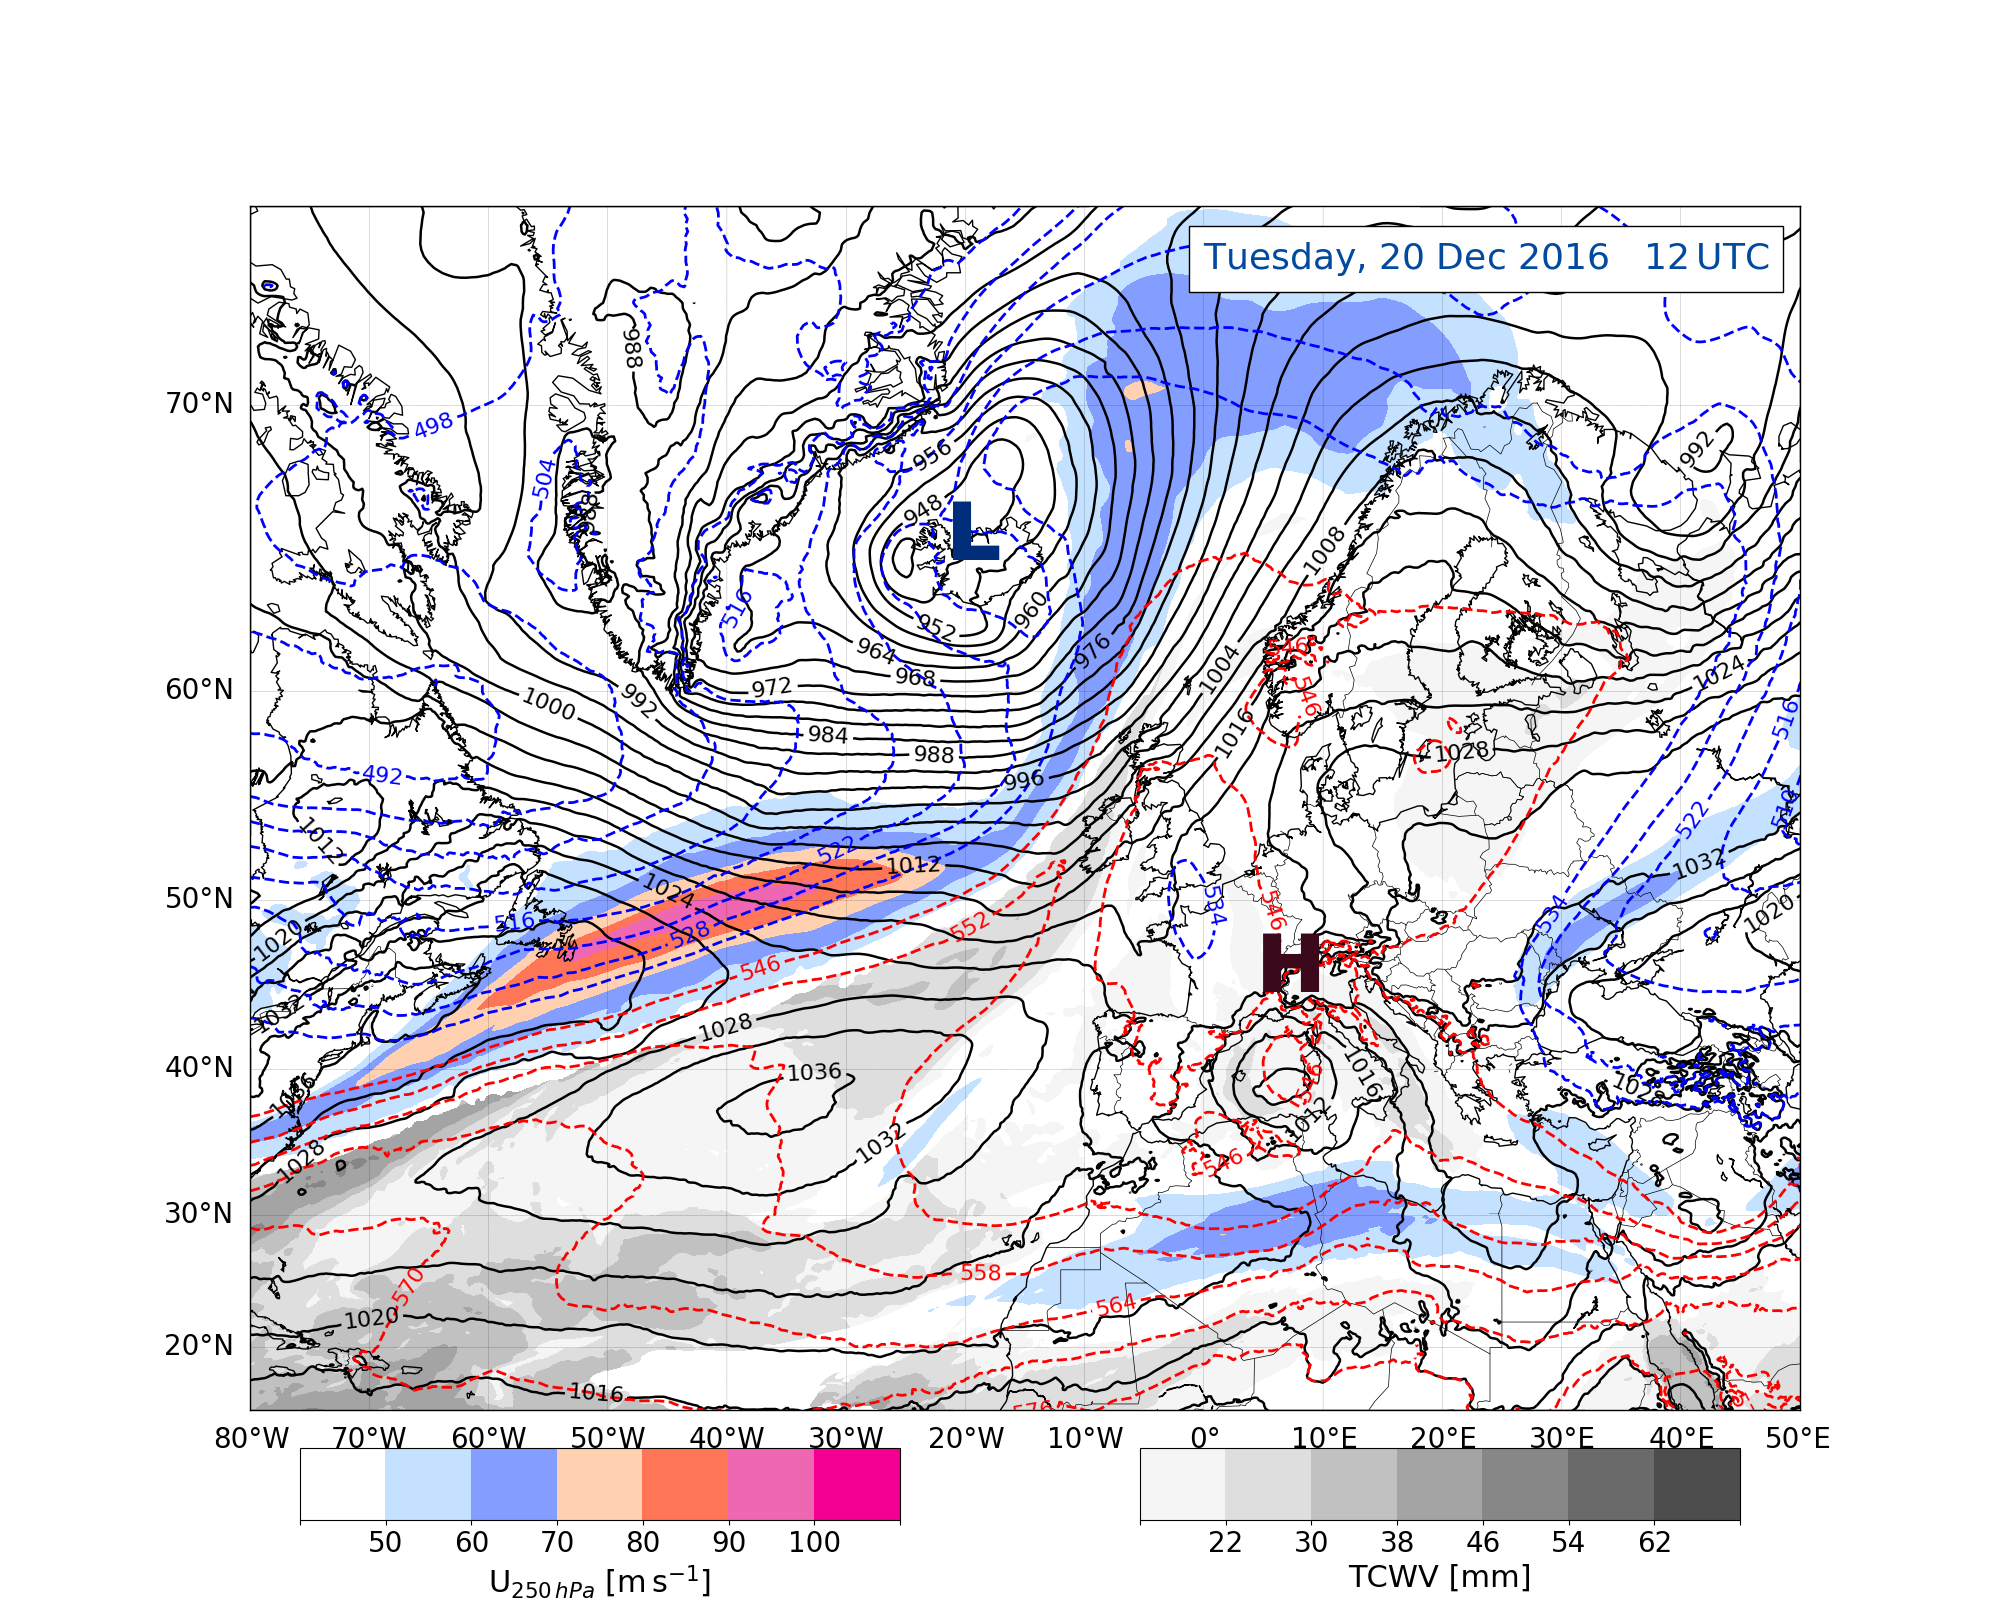
\includegraphics[trim={4.2cm 3.9cm 4.3cm 5.1cm},clip,
        width=\textwidth]{./fig_Geopot_Jet/20161220_12}
        \caption{}\label{fig:GP20}
        %\label{fig:DT2100}
    \end{subfigure}
%%%%%% 21/12
    \begin{subfigure}[b]{0.49\textwidth}
        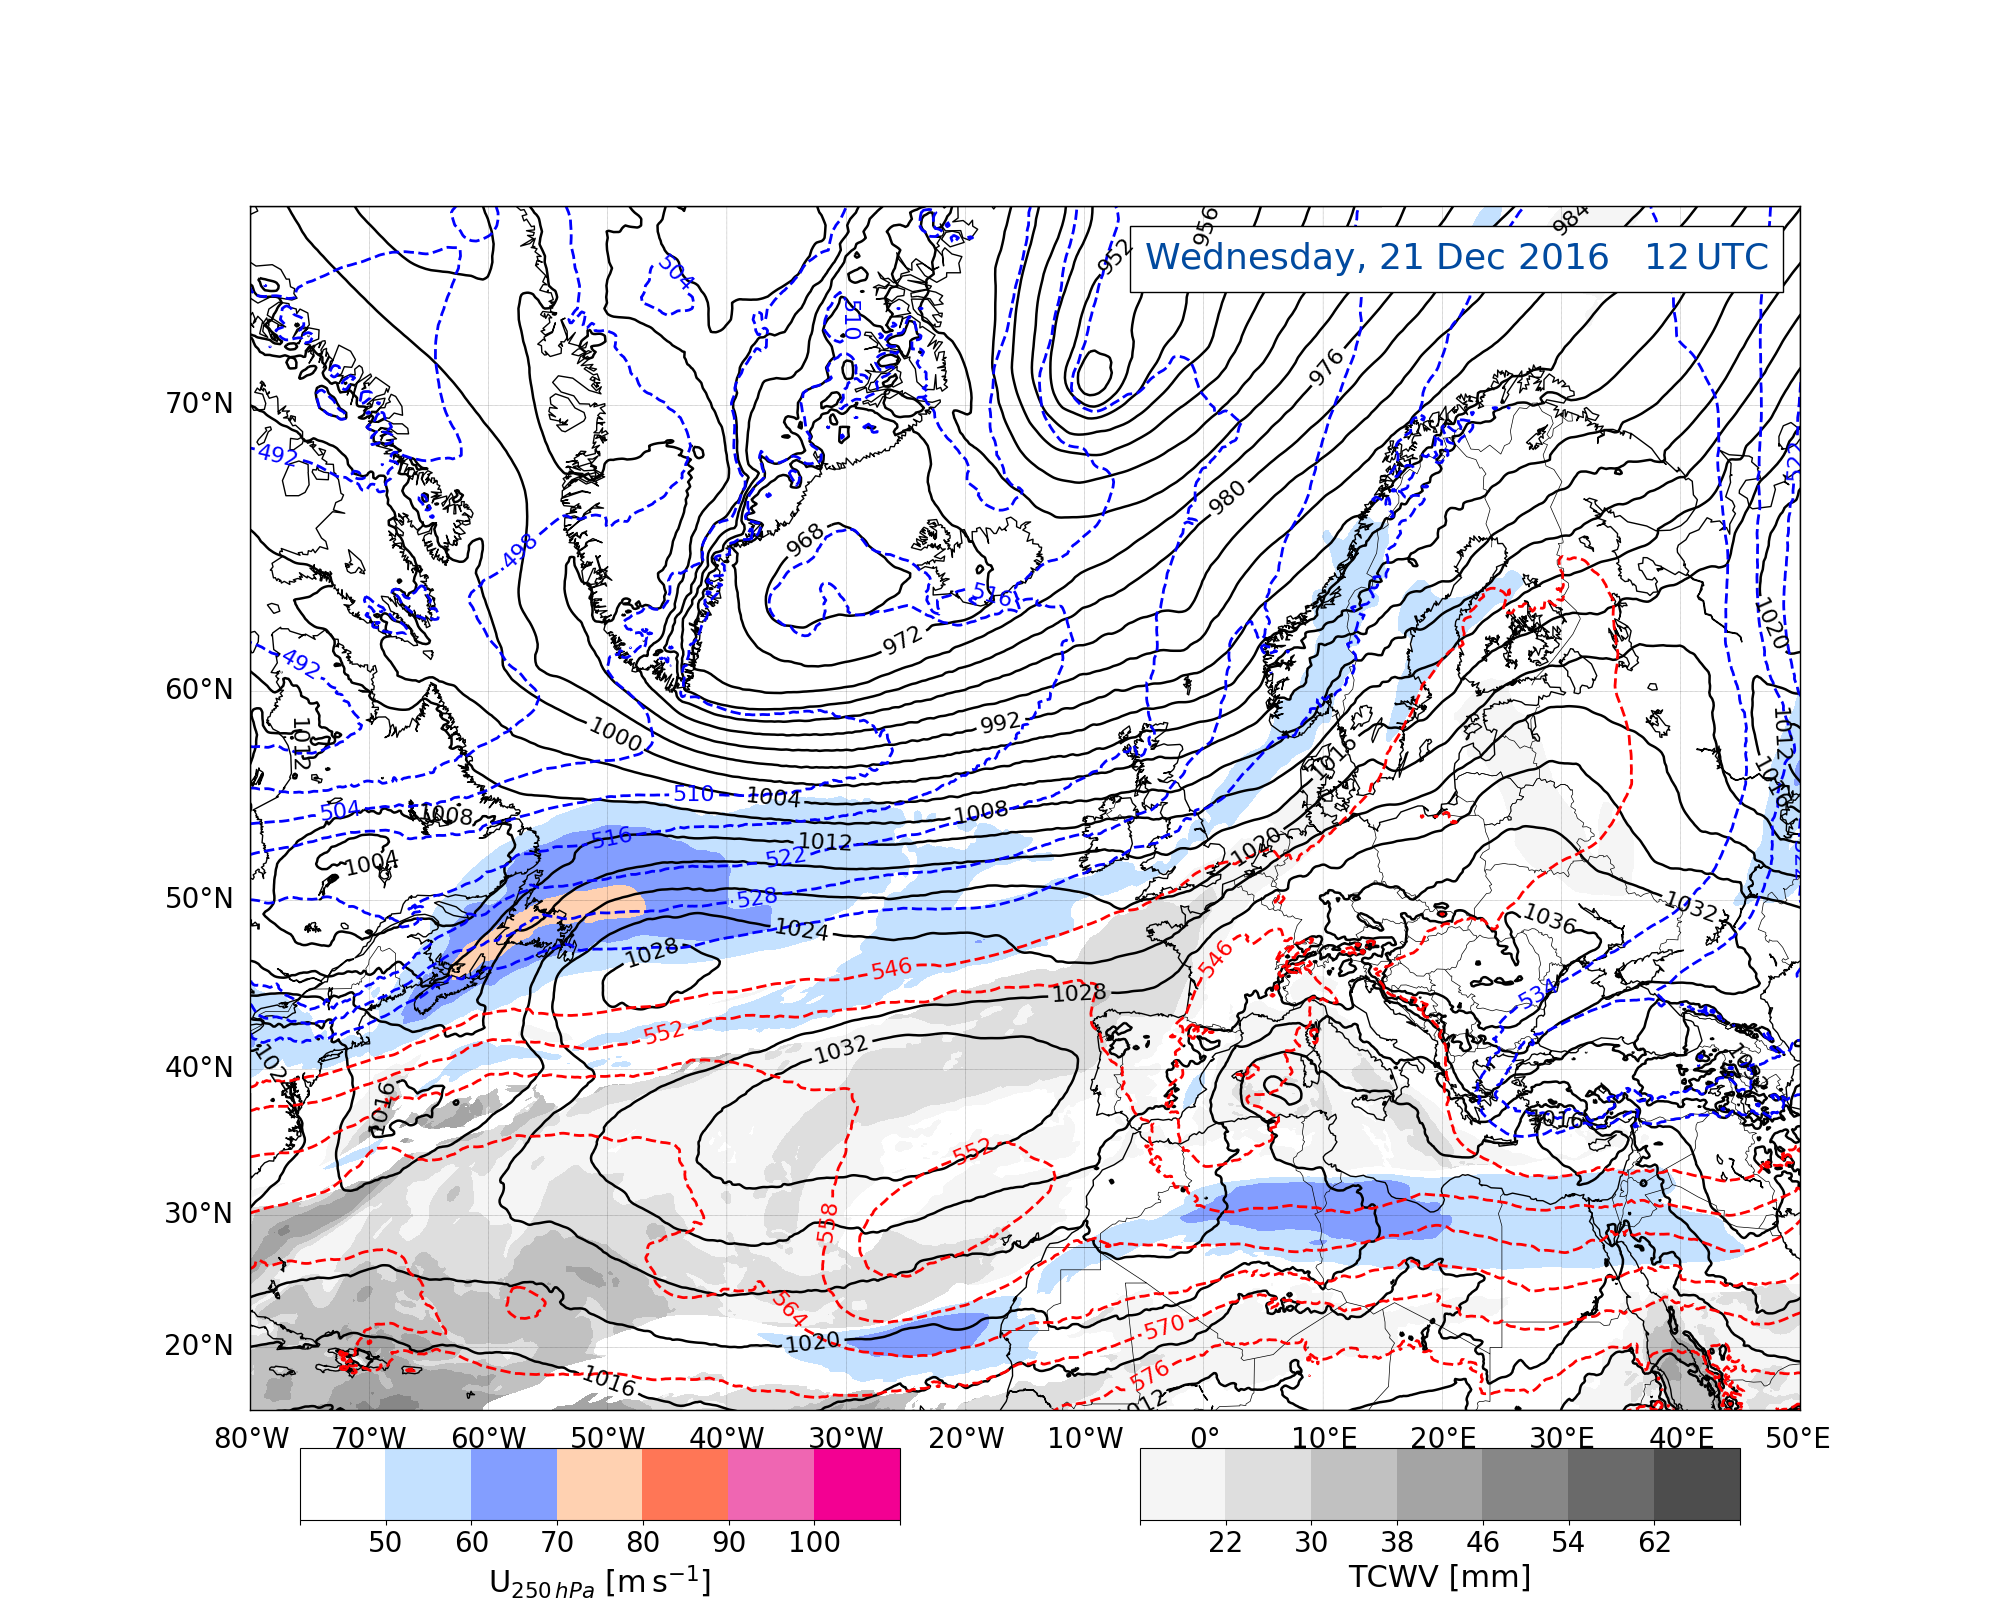
\includegraphics[trim={4.2cm 3.9cm 4.3cm 5.1cm},clip,
        width=\textwidth]{./fig_Geopot_Jet/20161221_12}
        \caption{}\label{fig:GP21}
    \end{subfigure}
%%%%%% 22/12
	\begin{subfigure}[b]{0.49\textwidth}
		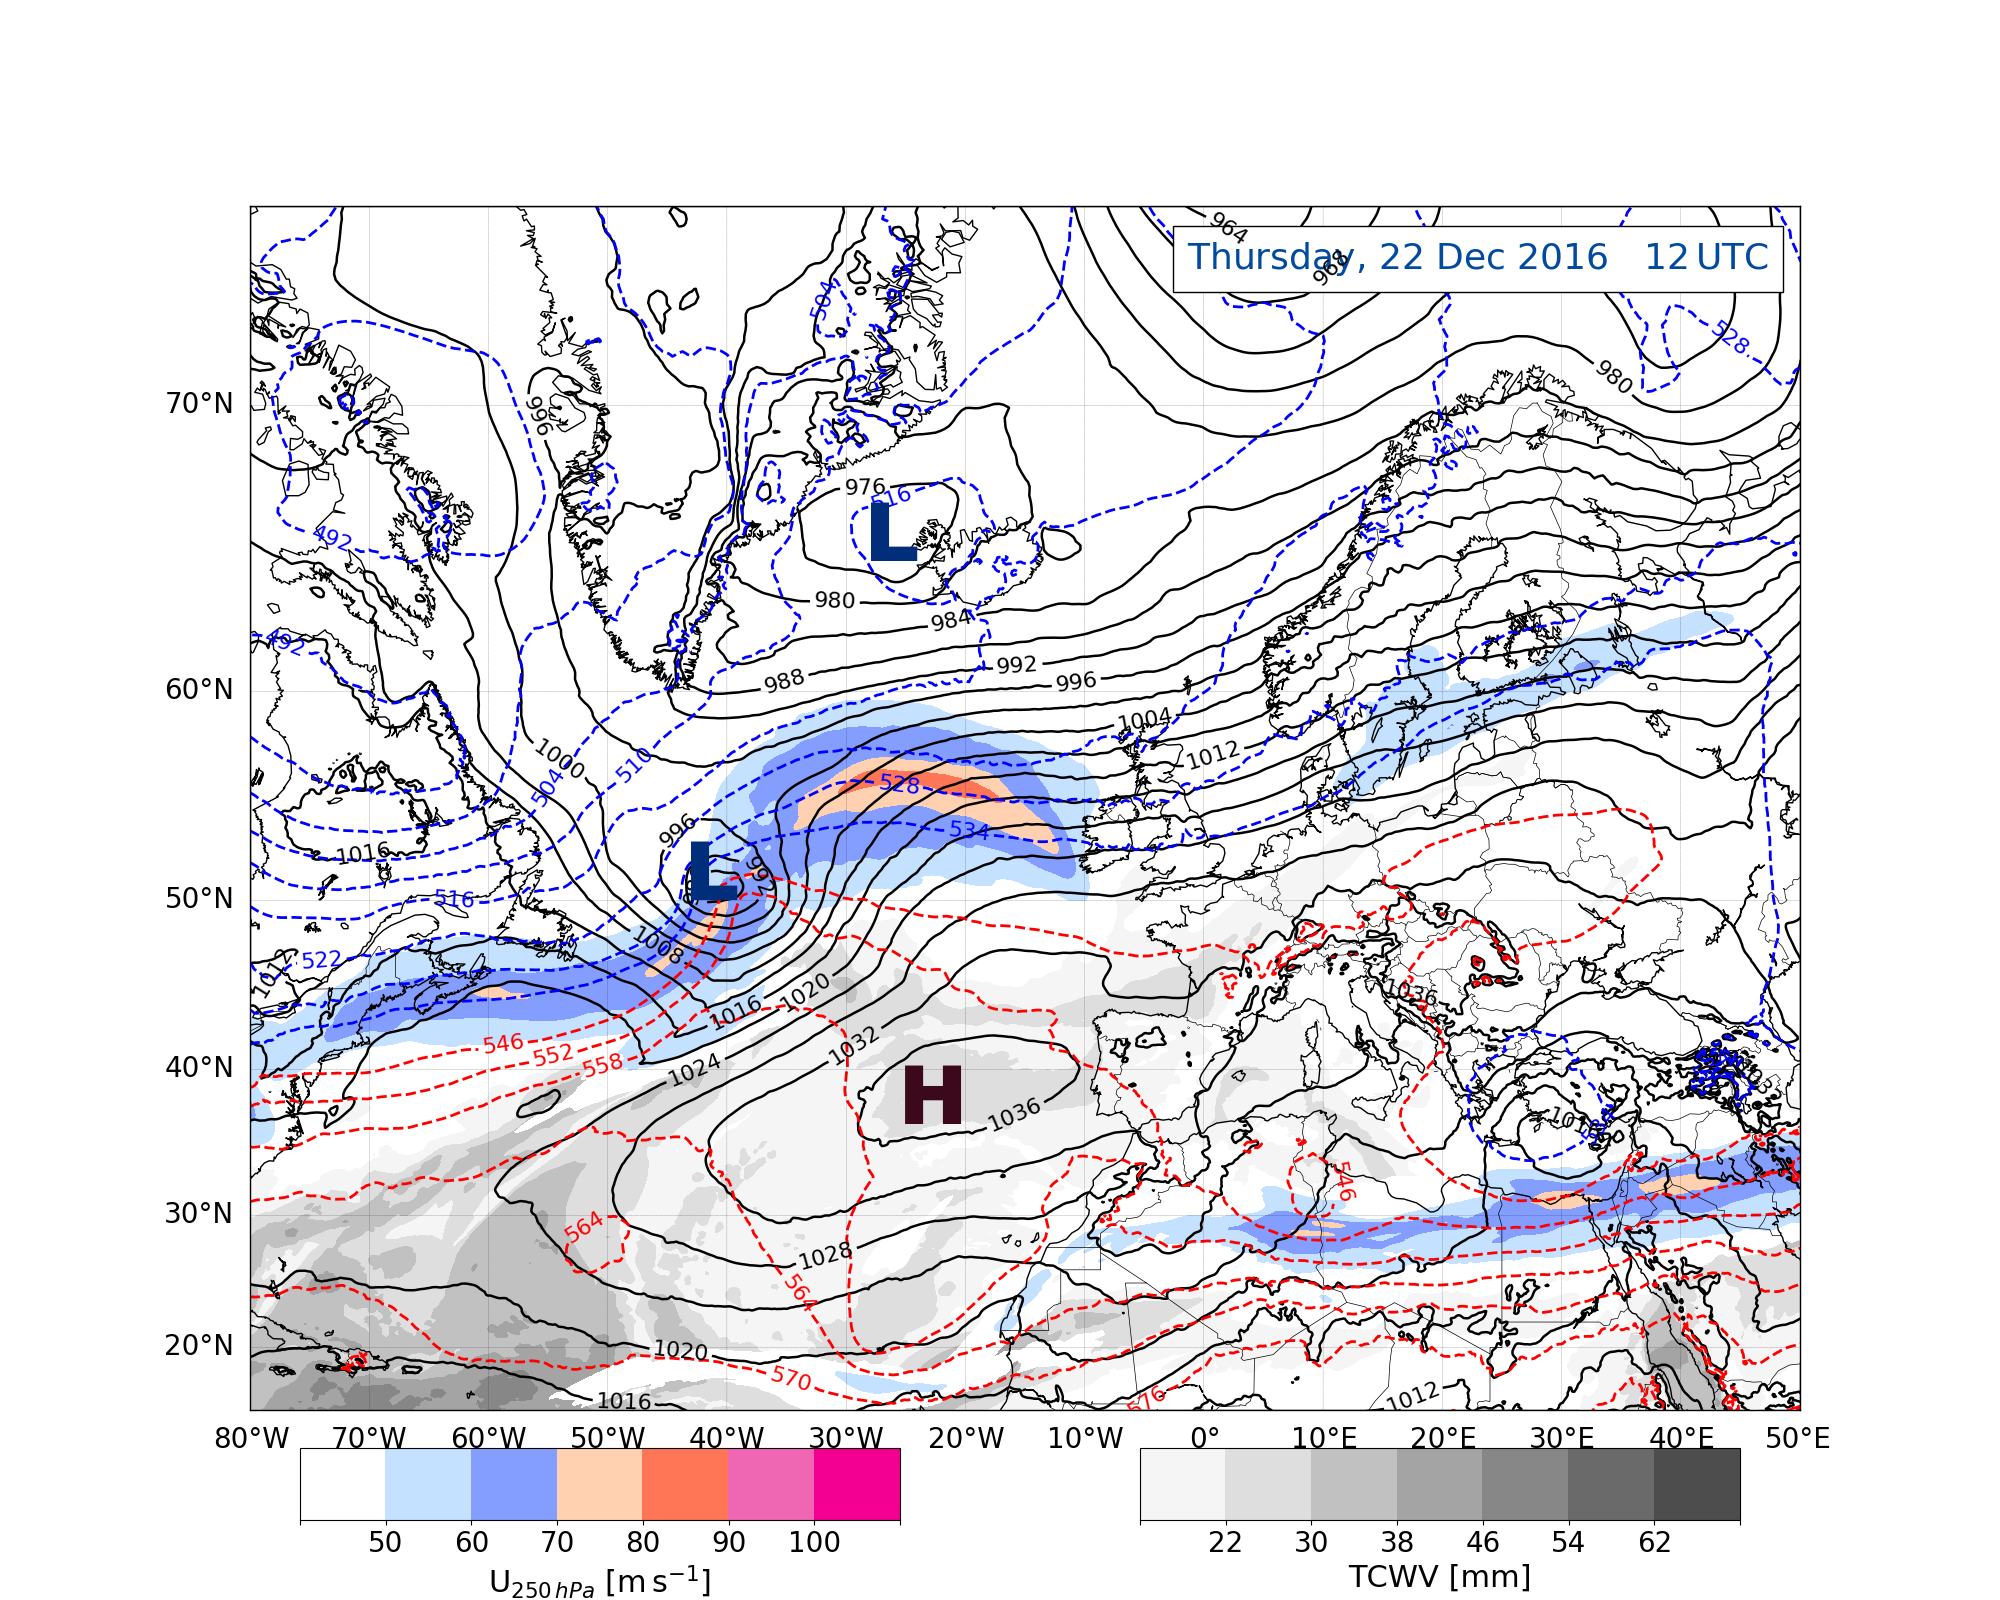
\includegraphics[trim={4.2cm 3.9cm 4.3cm 5.1cm},clip,
	width=\textwidth]{./fig_Geopot_Jet/20161222_12}
		\caption{}\label{fig:GP22}
	%\label{fig:sfc2100}
	\end{subfigure}
%%%%%% 23/12
	\begin{subfigure}[b]{0.49\textwidth}
		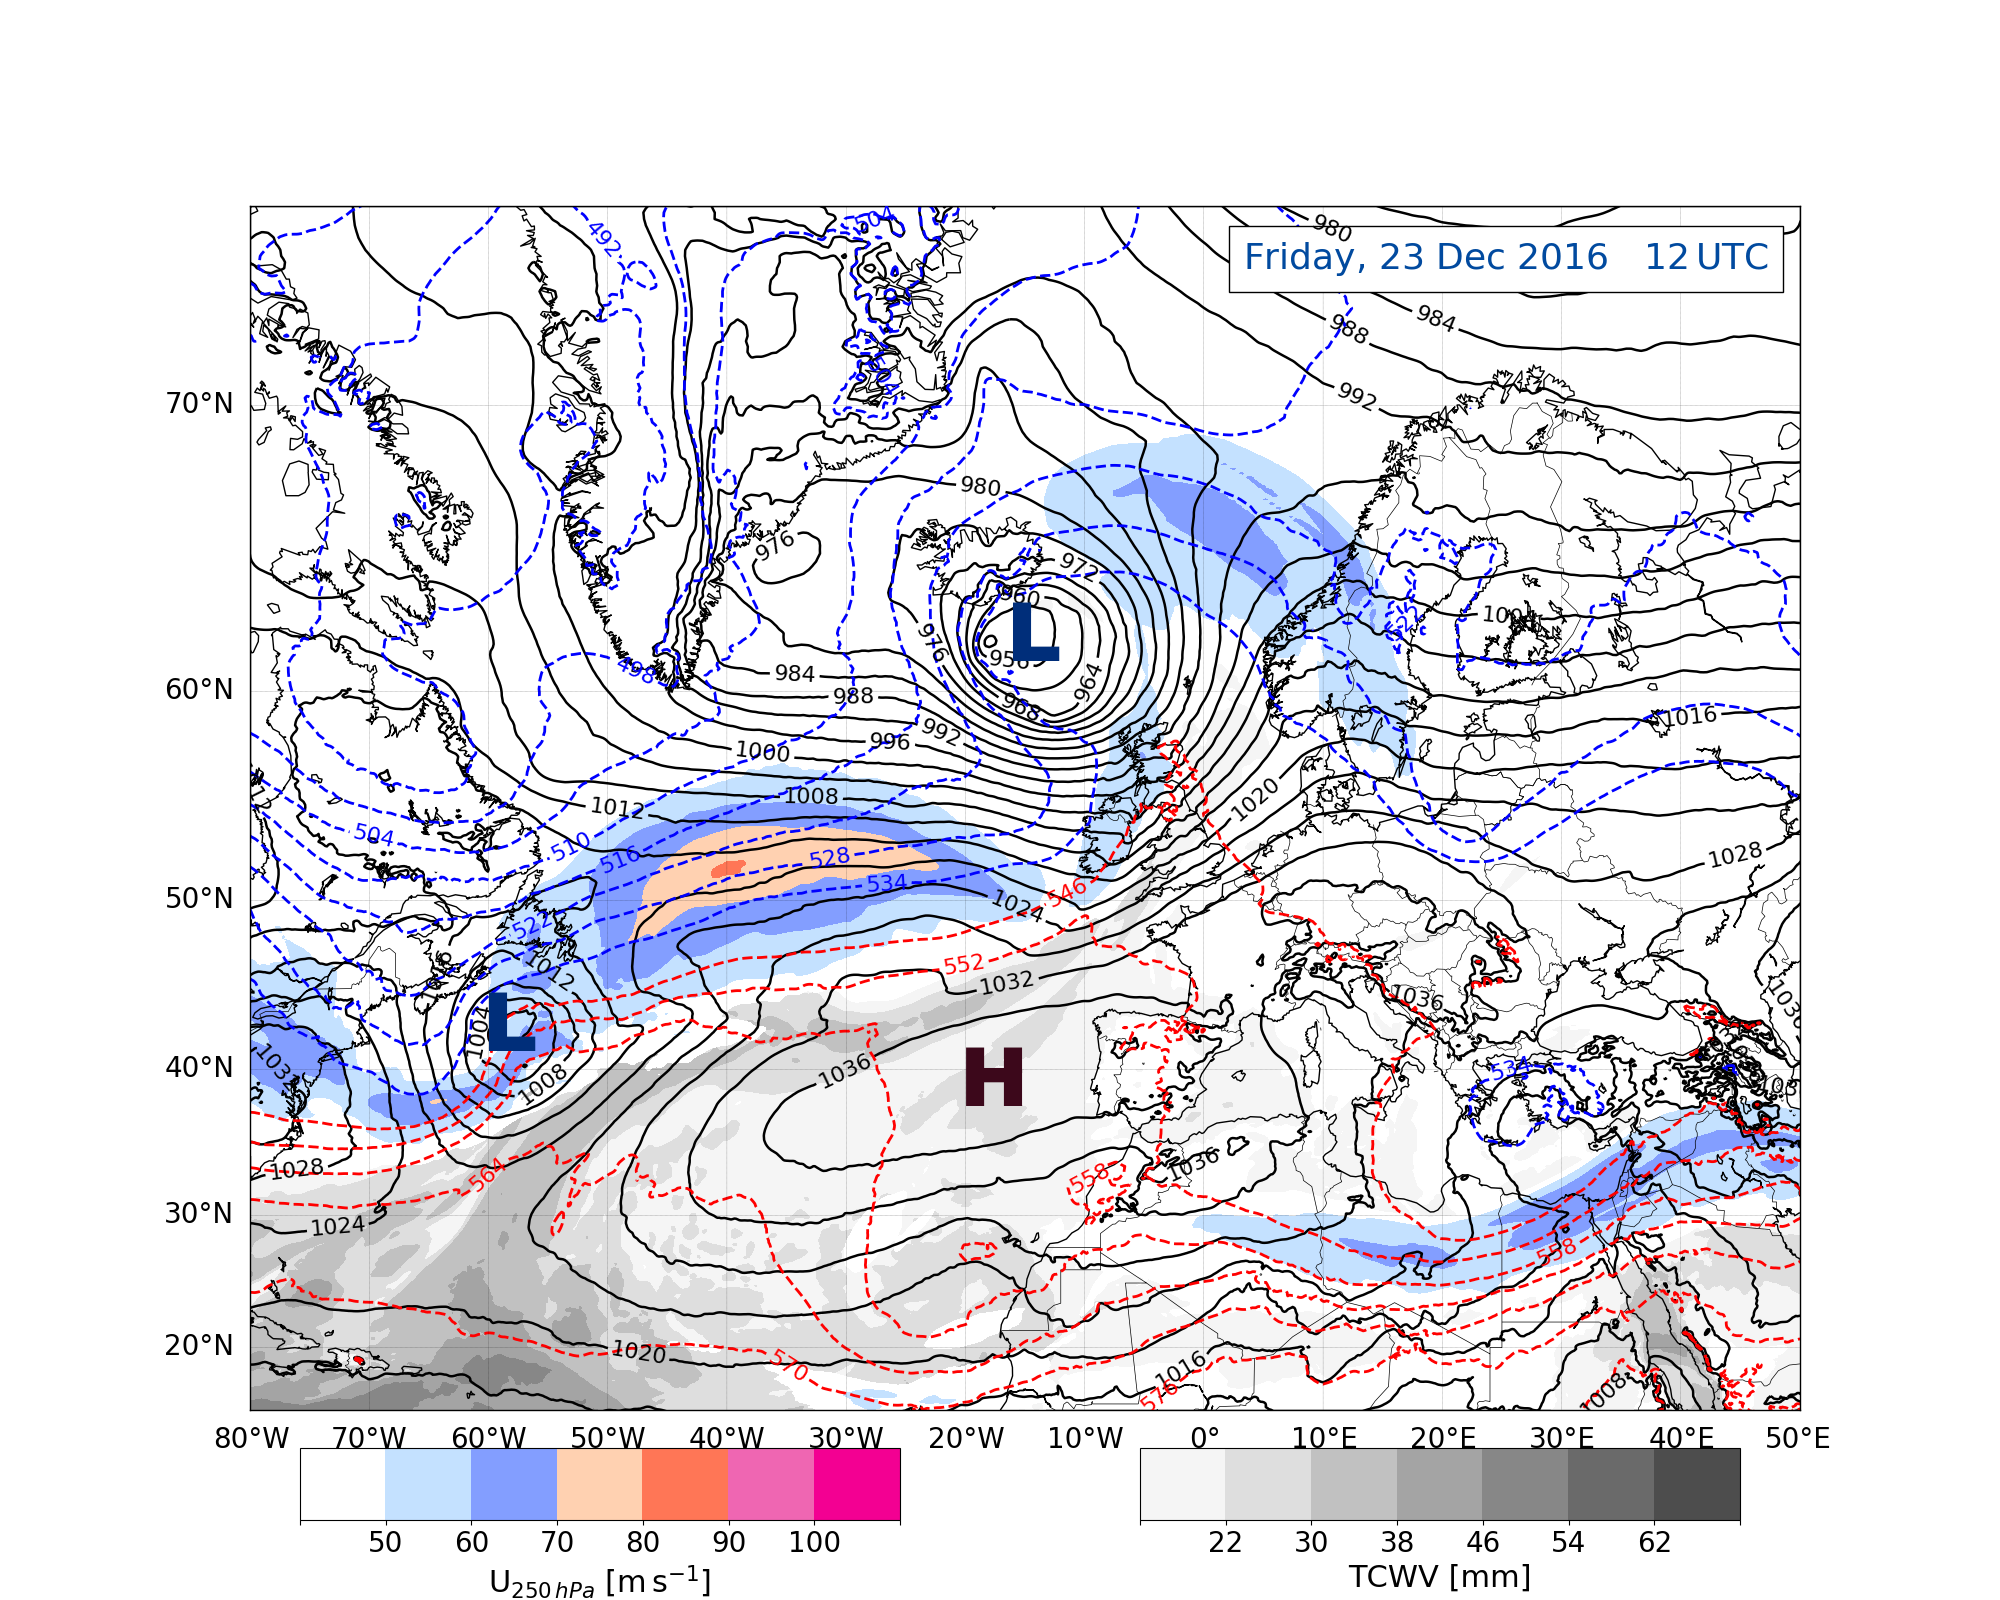
\includegraphics[trim={4.2cm 3.9cm 4.3cm 5.1cm},clip,
	width=\textwidth]{./fig_Geopot_Jet/20161223_12}
		\caption{}\label{fig:GP23}
	\end{subfigure}
%%%%%% label
    \begin{subfigure}[b]{\textwidth}
        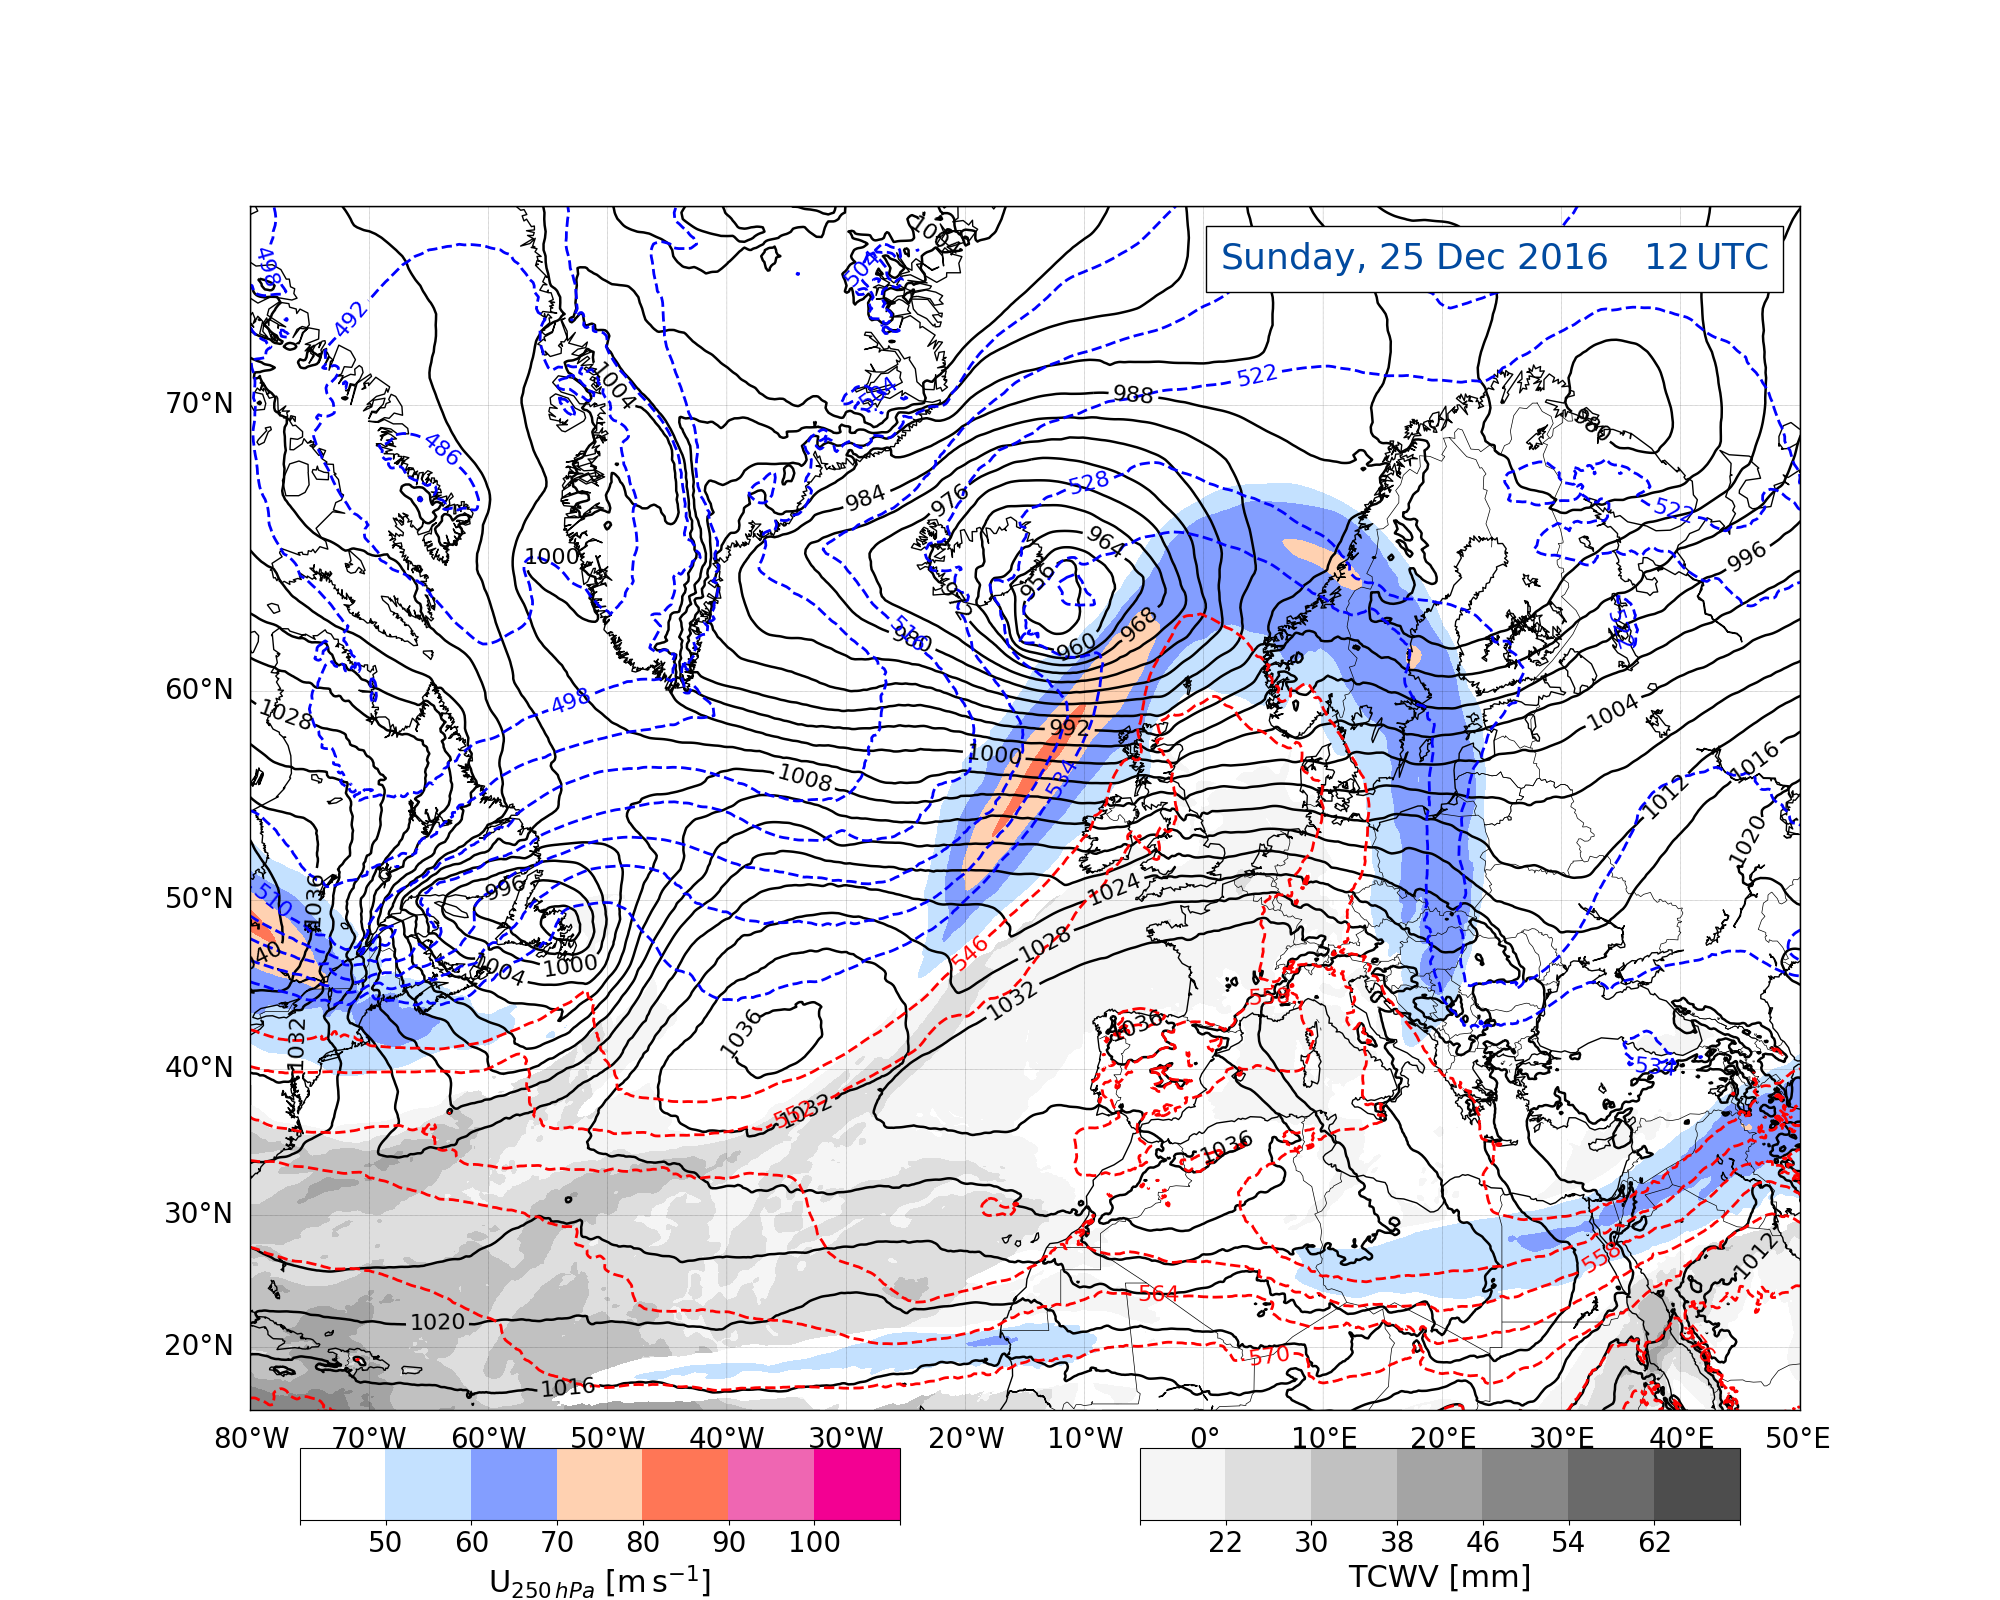
\includegraphics[trim={4.2cm 0cm 4.3cm 36.8cm},clip,
        width=\textwidth]{./fig_Geopot_Jet/20161225_12}
    \end{subfigure}
\caption{Jet, thickness, mean sea level pressure, and moisture synoptic analysis, data from ECMWF. During \SIrange{20}{27}{\dec}. \SI{250}{\hPa} wind speed, shaded according to the colour bar, [\SI{}{\mPs}]. \SI{1000}-\SI{500}{\hPa} thickness, dashed contours every \SI{6}{\deca\meter}, MSLP, black contours every \SI{4}{\hPa}, total column water vapour [\SI{}{\mm}], shaded according the grey scale.}\label{fig:GeopJet}
\end{figure}
\begin{figure}\ContinuedFloat
	\centering
%%%%%% 24/12
    \begin{subfigure}[b]{0.49\textwidth}
        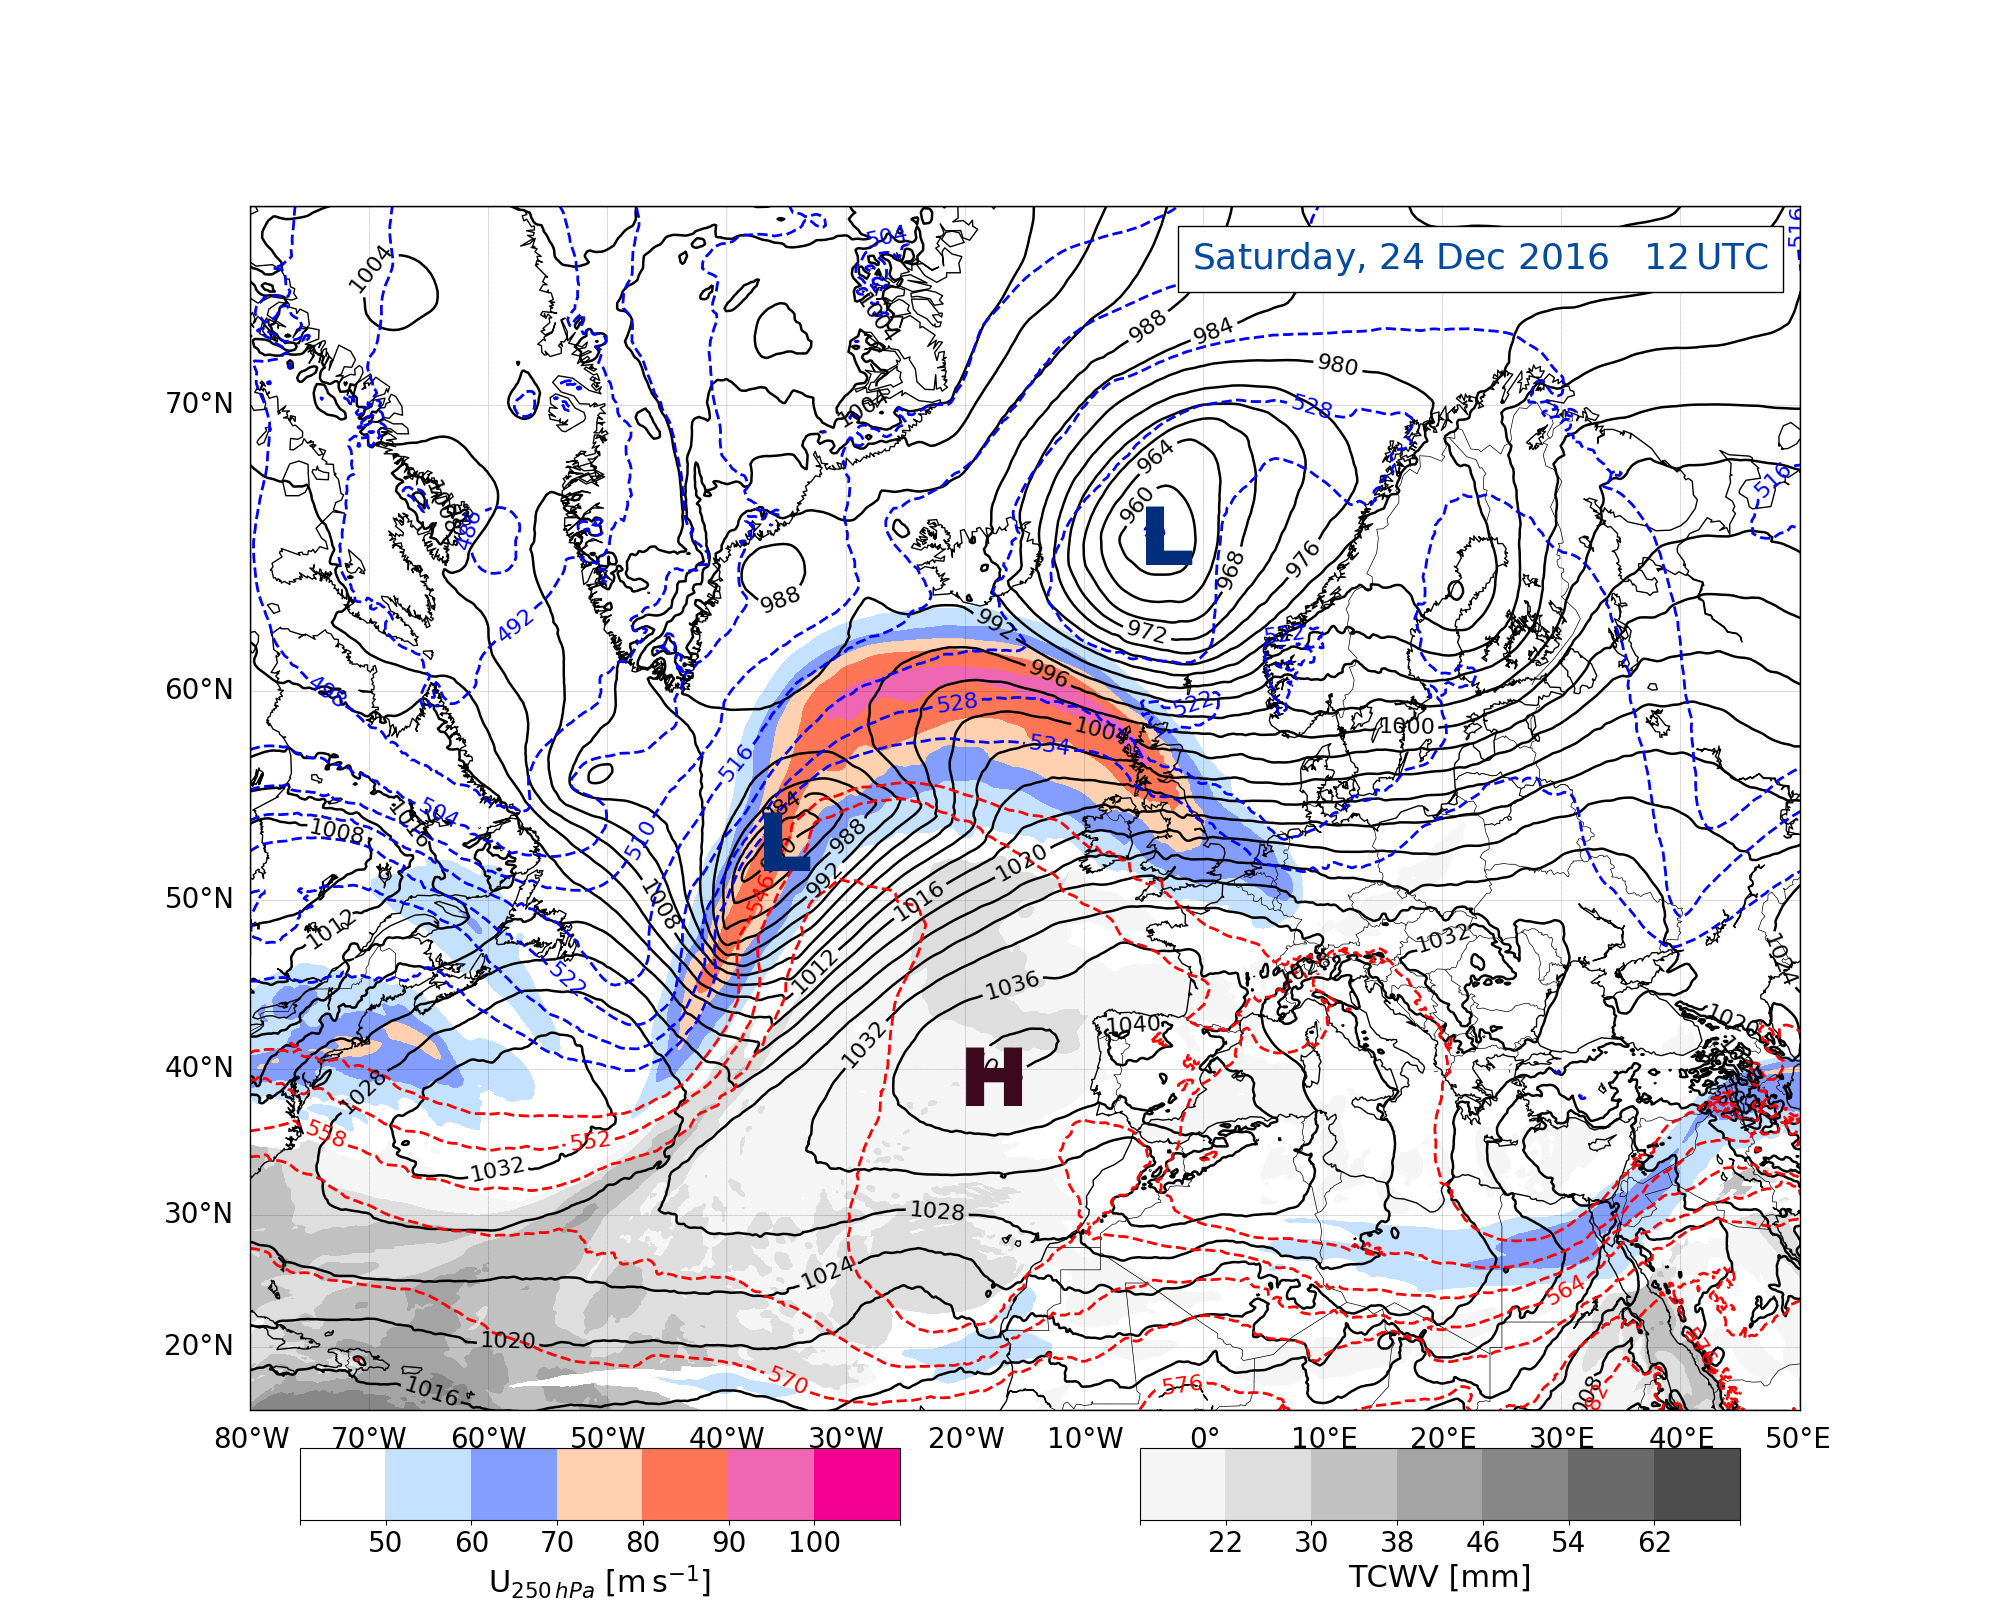
\includegraphics[trim={4.2cm 3.9cm 4.3cm 5.1cm},clip,
        width=\textwidth]{./fig_Geopot_Jet/20161224_12}
        \caption{}\label{fig:GP24}
    \end{subfigure}
%%%%%% 25/12
    \begin{subfigure}[b]{0.49\textwidth}
        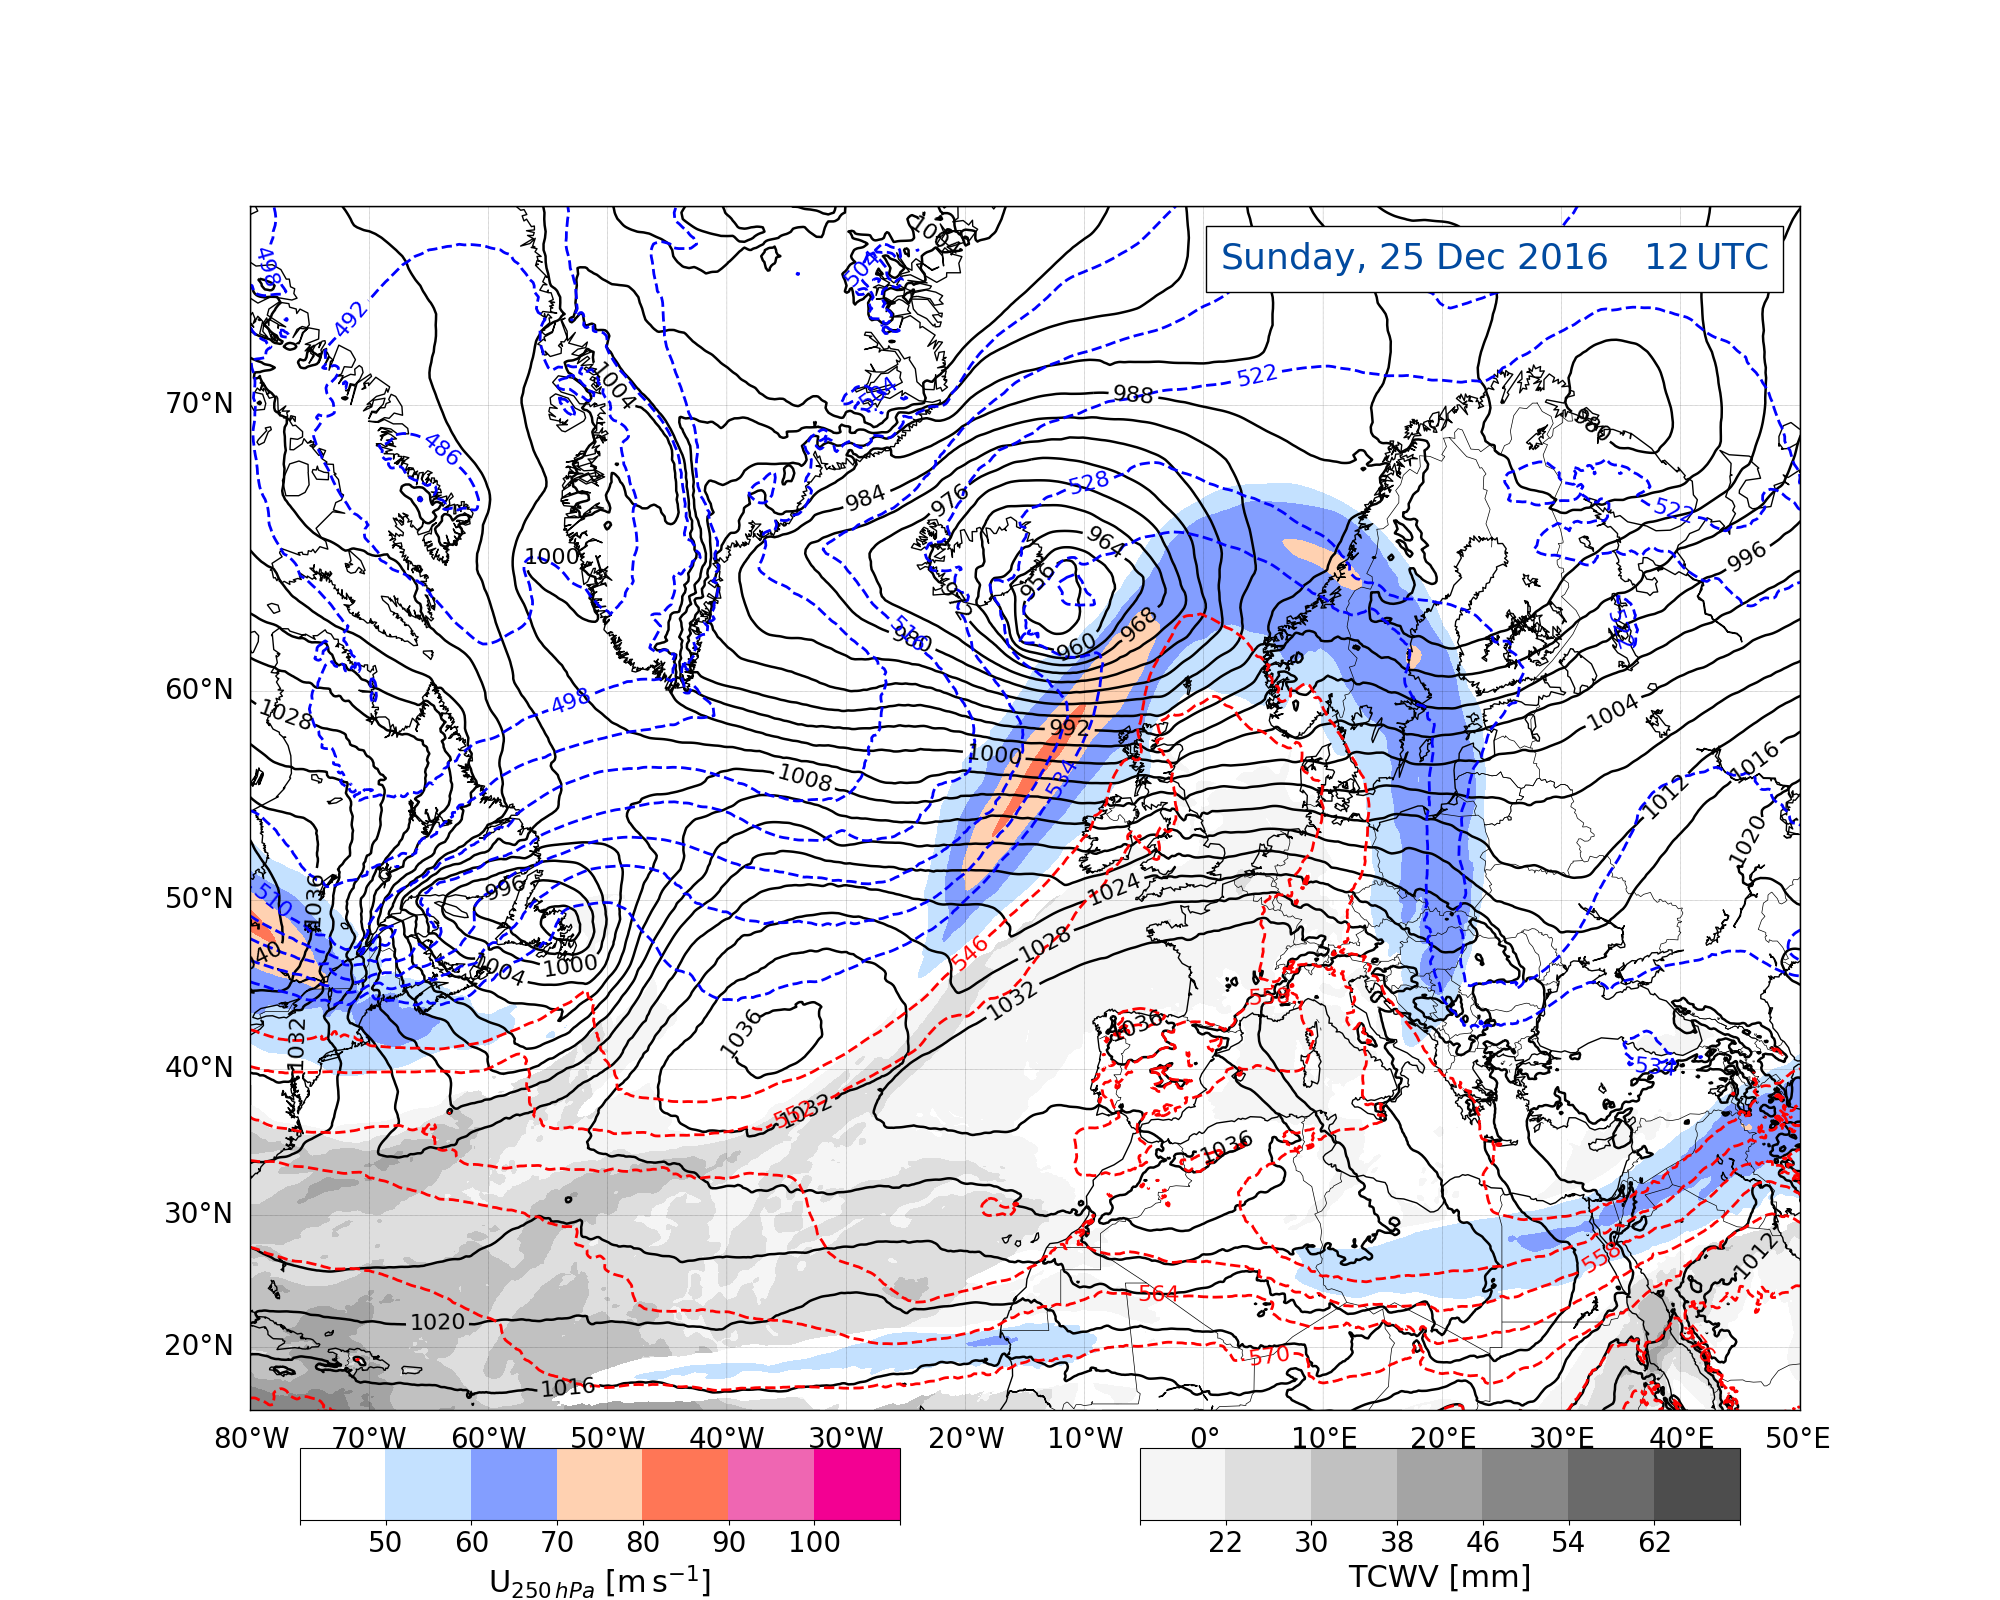
\includegraphics[trim={4.2cm 3.9cm 4.3cm 5.1cm},clip,
        width=\textwidth]{./fig_Geopot_Jet/20161225_12}
        \caption{}\label{fig:GP25}
    \end{subfigure}
%	\centering
%%%%%% 26/12
    \begin{subfigure}[b]{0.49\textwidth}
        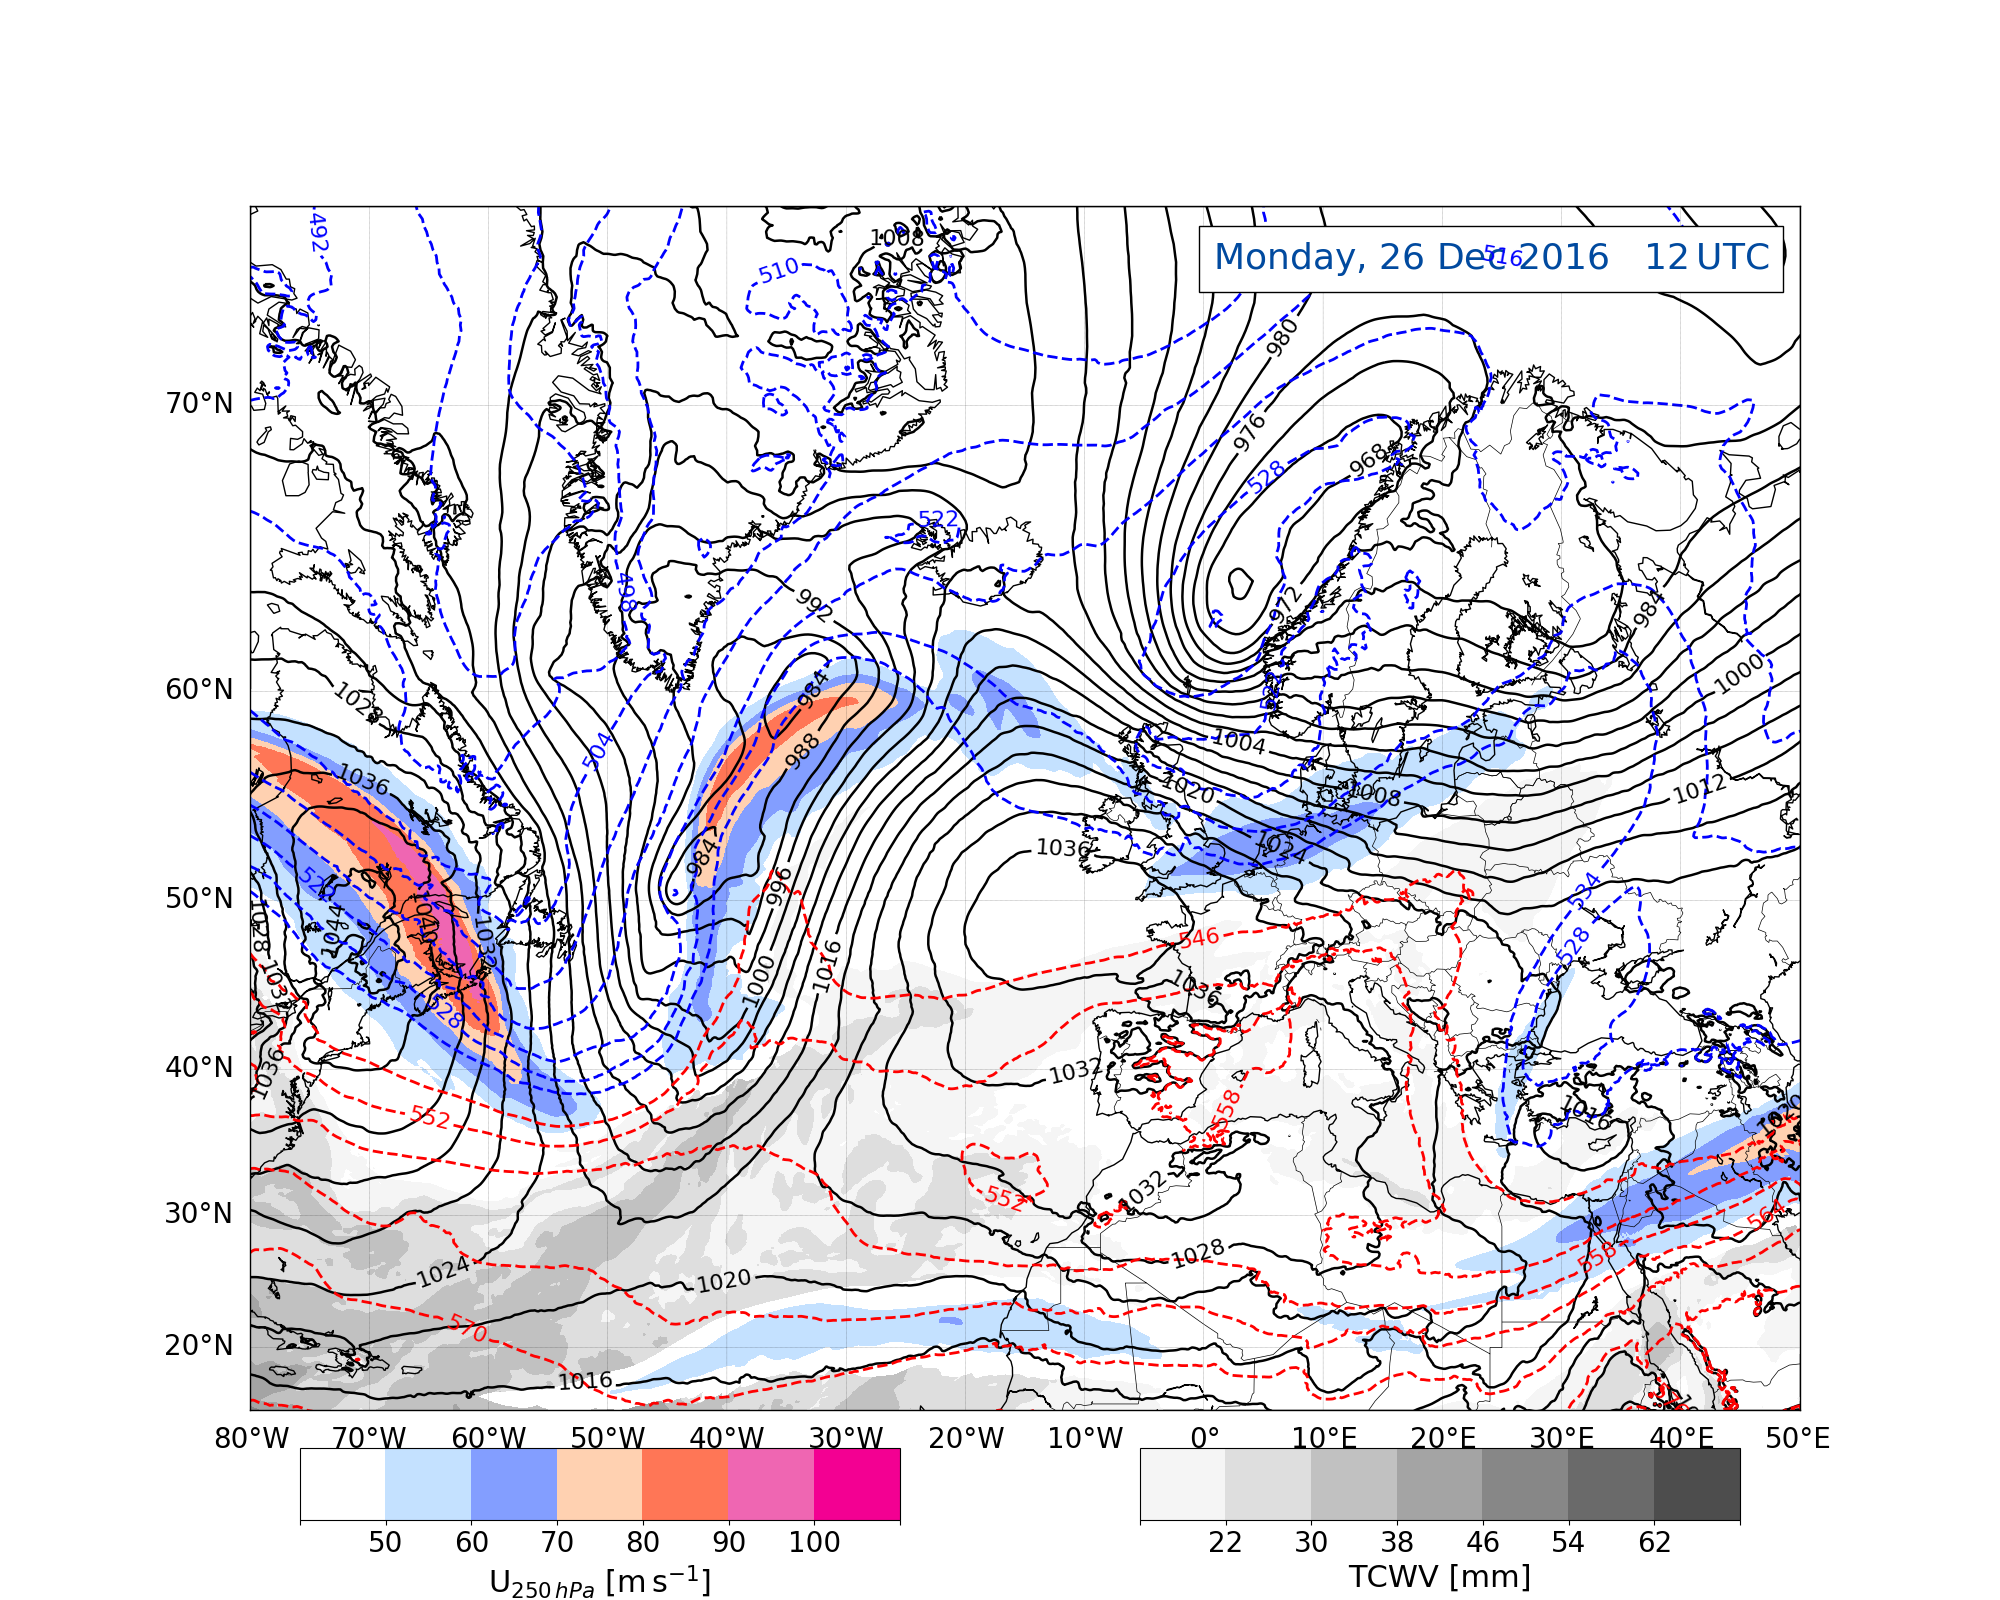
\includegraphics[trim={4.2cm 3.9cm 4.3cm 5.1cm},clip,
        width=\textwidth]{./fig_Geopot_Jet/20161226_12}
        \caption{}\label{fig:GP26}
    \end{subfigure}
%%%%%% 27/12
    \begin{subfigure}[b]{0.49\textwidth}
        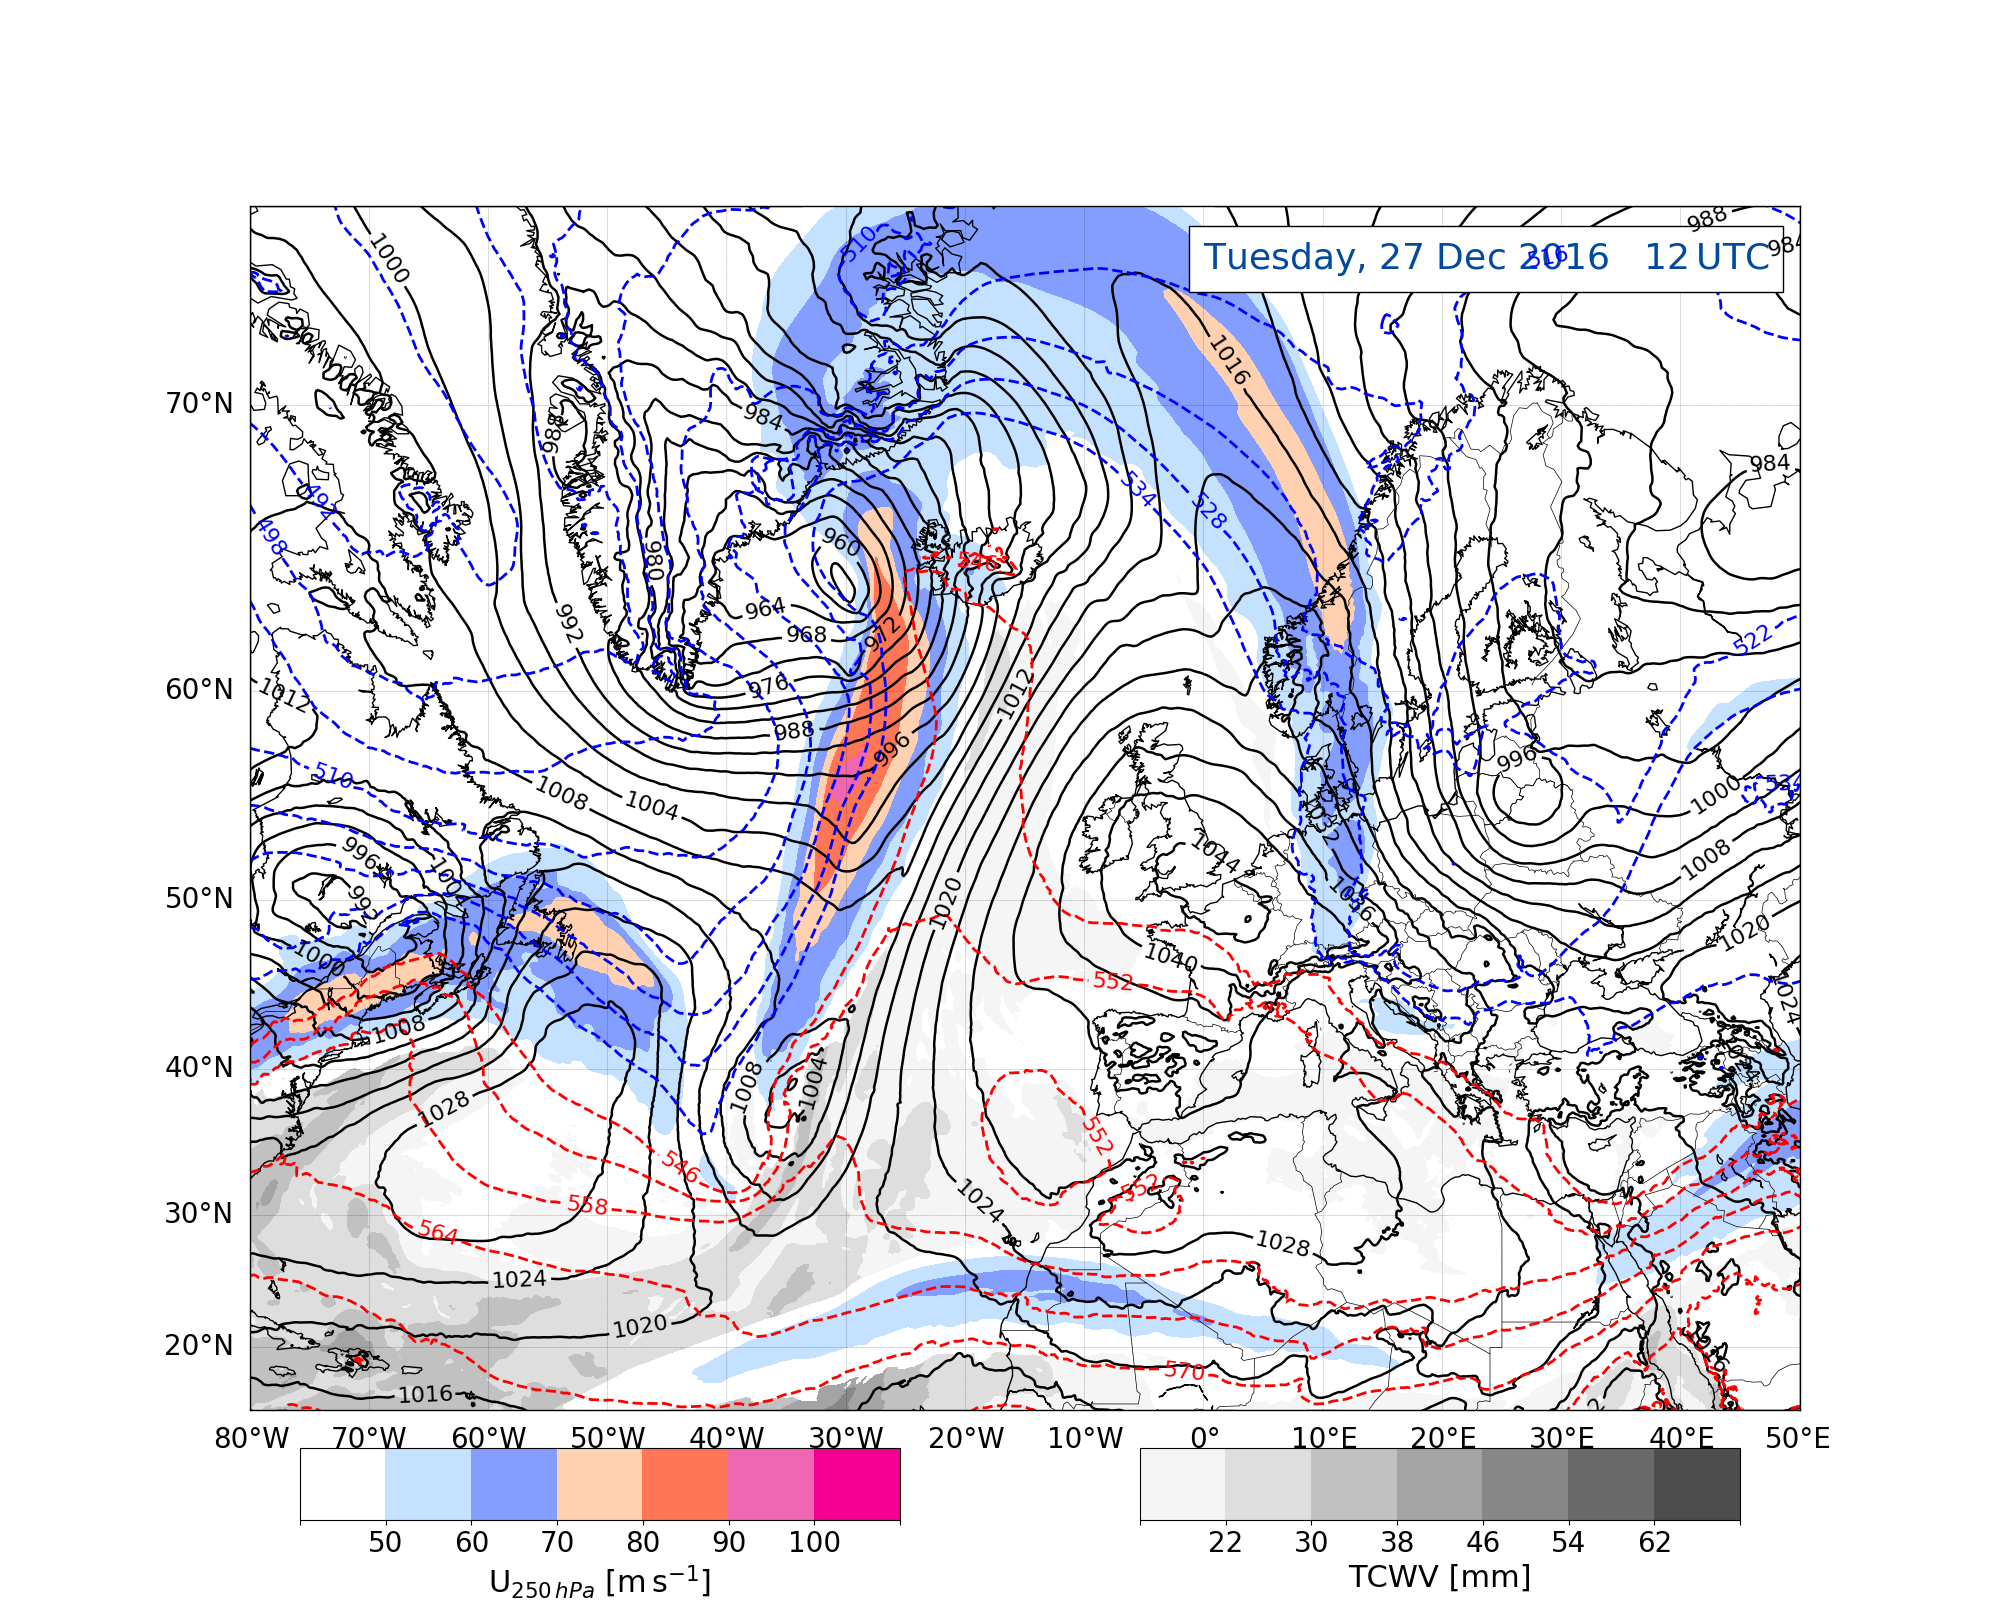
\includegraphics[trim={4.2cm 3.9cm 4.3cm 5.1cm},clip,
        width=\textwidth]{./fig_Geopot_Jet/20161227_12}
        \caption{}\label{fig:GP27}
    \end{subfigure}
%%%%%% label
    \begin{subfigure}[b]{\textwidth}
        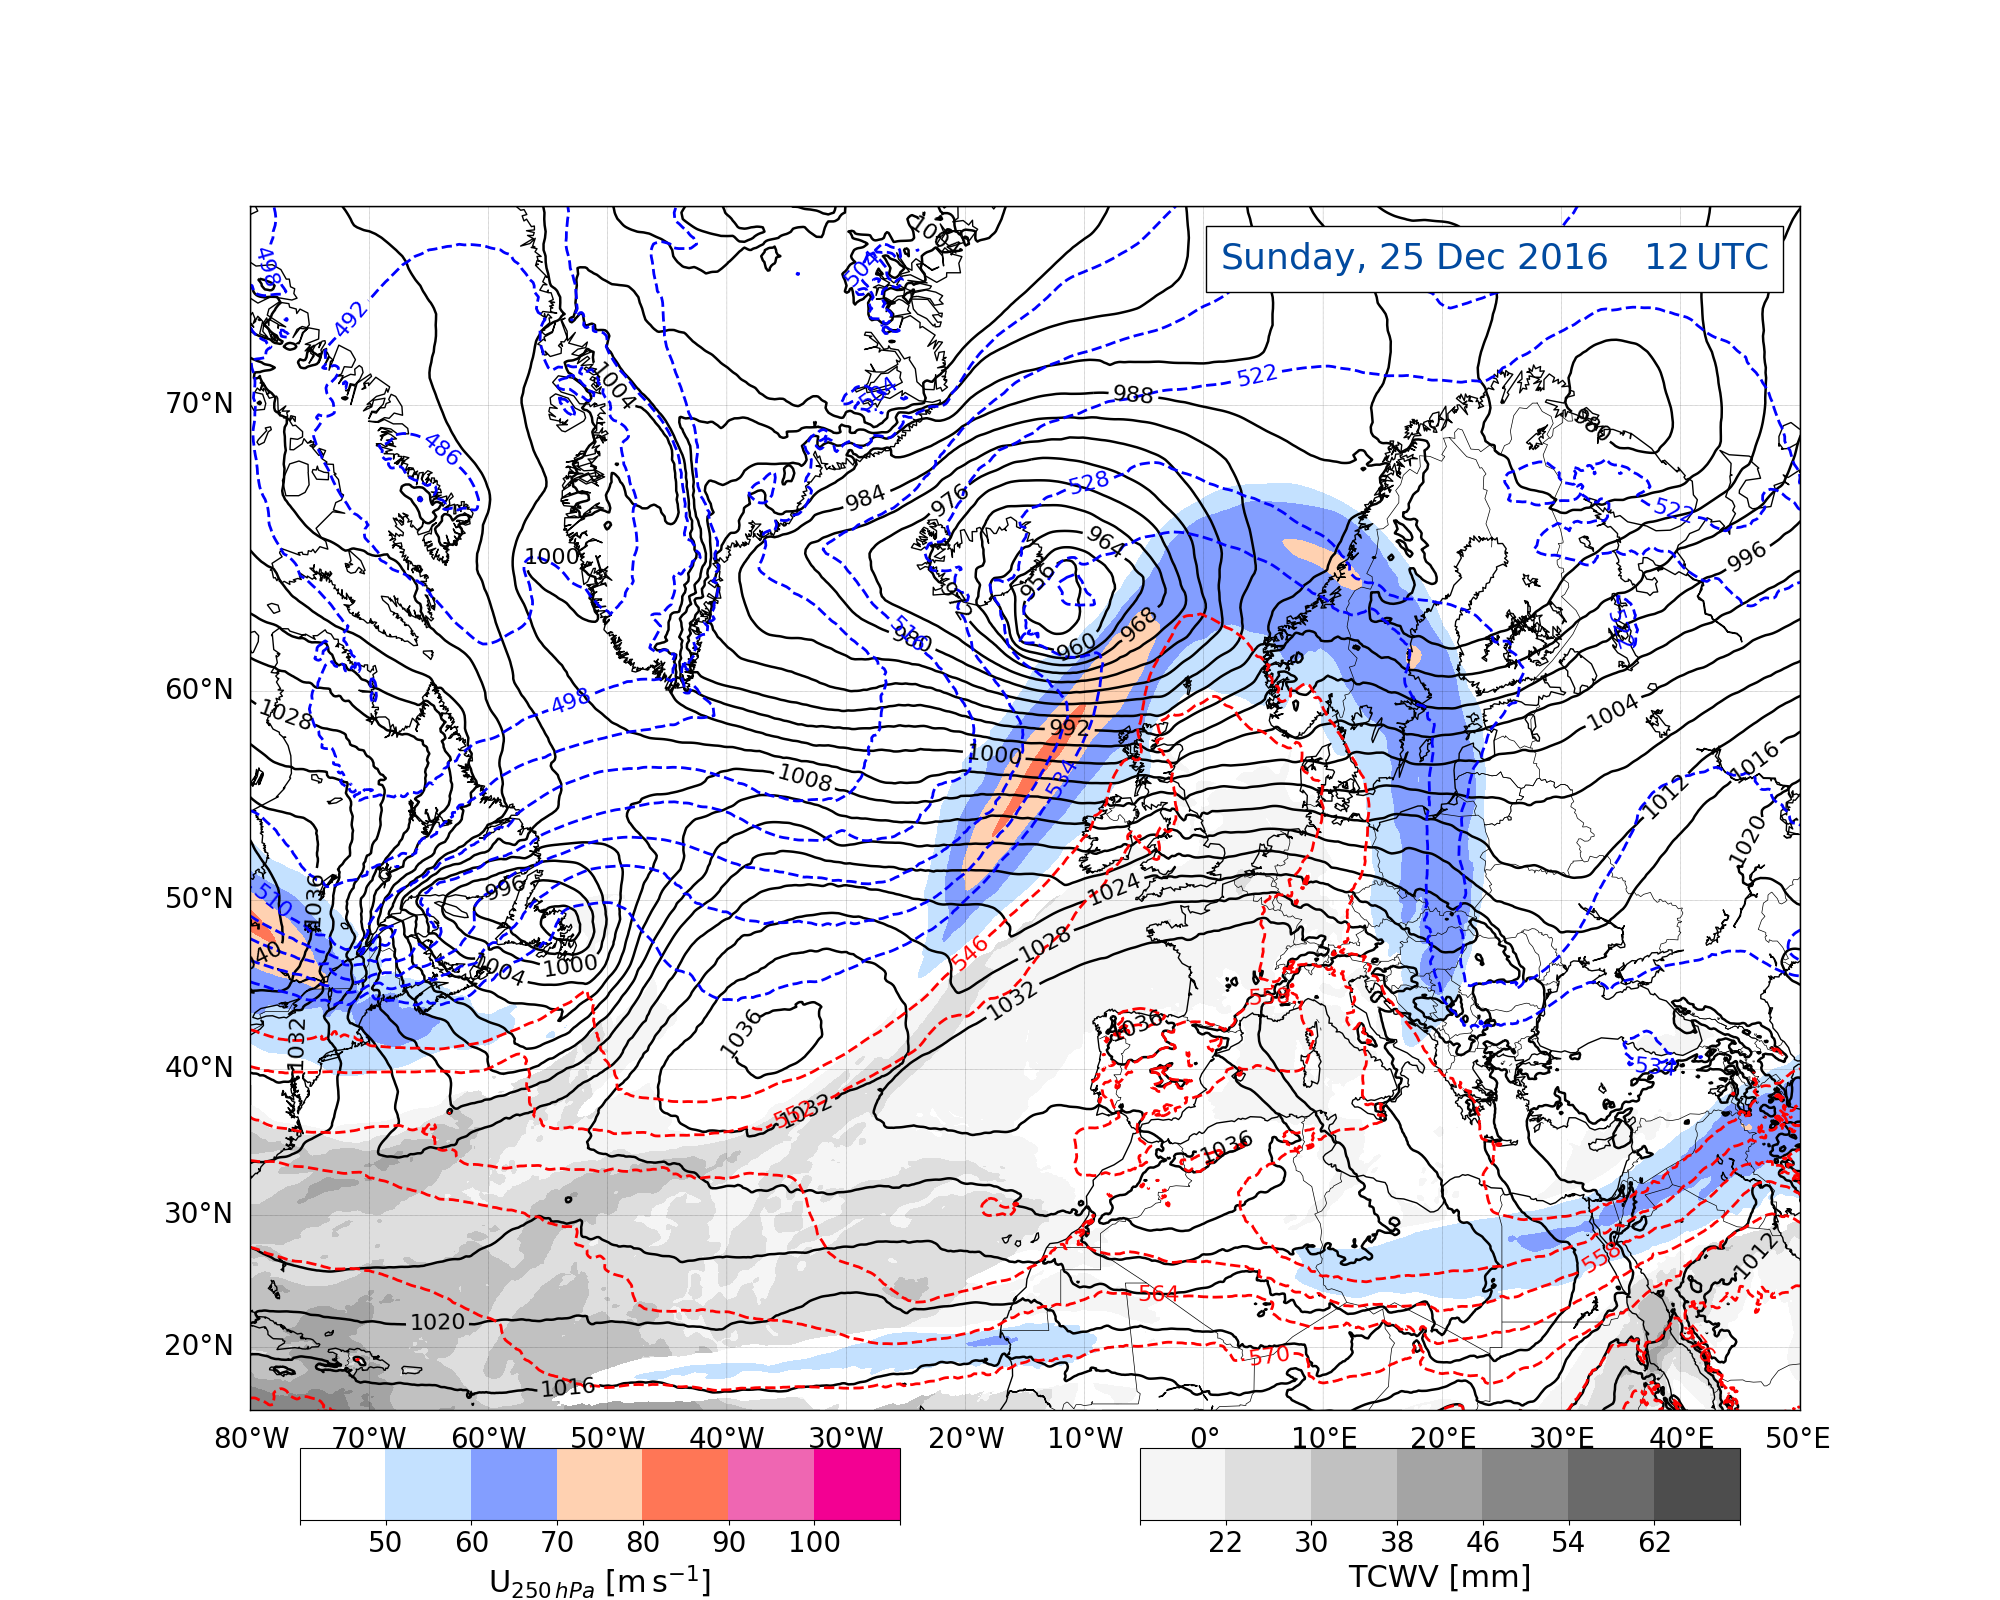
\includegraphics[trim={4.2cm 0cm 4.3cm 36.8cm},clip,
        width=\textwidth]{./fig_Geopot_Jet/20161225_12}
       % \label{fig:D}
    \end{subfigure}
\caption{\textit{(Continued from previous page.)}}   
\end{figure}
%%%%%%%%%%%%%%%%%%%%%%%%%%%%%%%%%%%%%%%%%%%%%%%%%%%%%%%%%%%%%%%%%%%%%%%%%%
\noindent The dashed, coloured contours show the vertical thickness between the \SI{1000}{\hPa} and \SI{500}{\hPa} surface, every \SI{6}{\deca\meter}. The thickness between two pressure levels can be related to the hypsometric equation (\Cref{eq:hypsometric}). This is a relation of the mean temperature of the air between two pressure levels. Thus, high values of thickness mean relative warm, moist air (red, dashed). This can then be associated to rain or snow in mid-latitudes, depending on cold or warm air advection.
\\
Gray shaded areas describe total precipitable water in the atmosphere in \SI{}{\mm}. It is an indicator for the amount of moisture to supply rainfall, and will be used to identify where moisture was present.
\\
Colour shaded contours in \Cref{fig:GeopJet} indicate the mid-latitudal jet streaks at \SI{250}{\hPa}. Warmer colour is associated with higher wind speeds at this level.  
%%% Geopot Jet maps %%%%%%%%%%%%%%%%%%%%%%%%%%%%%%%%%%%%%
%% !TeX spellcheck = en_GB

\begin{figure}[h!]
    \centering
%%%%%% 20/12
    \begin{subfigure}[b]{0.49\textwidth}
        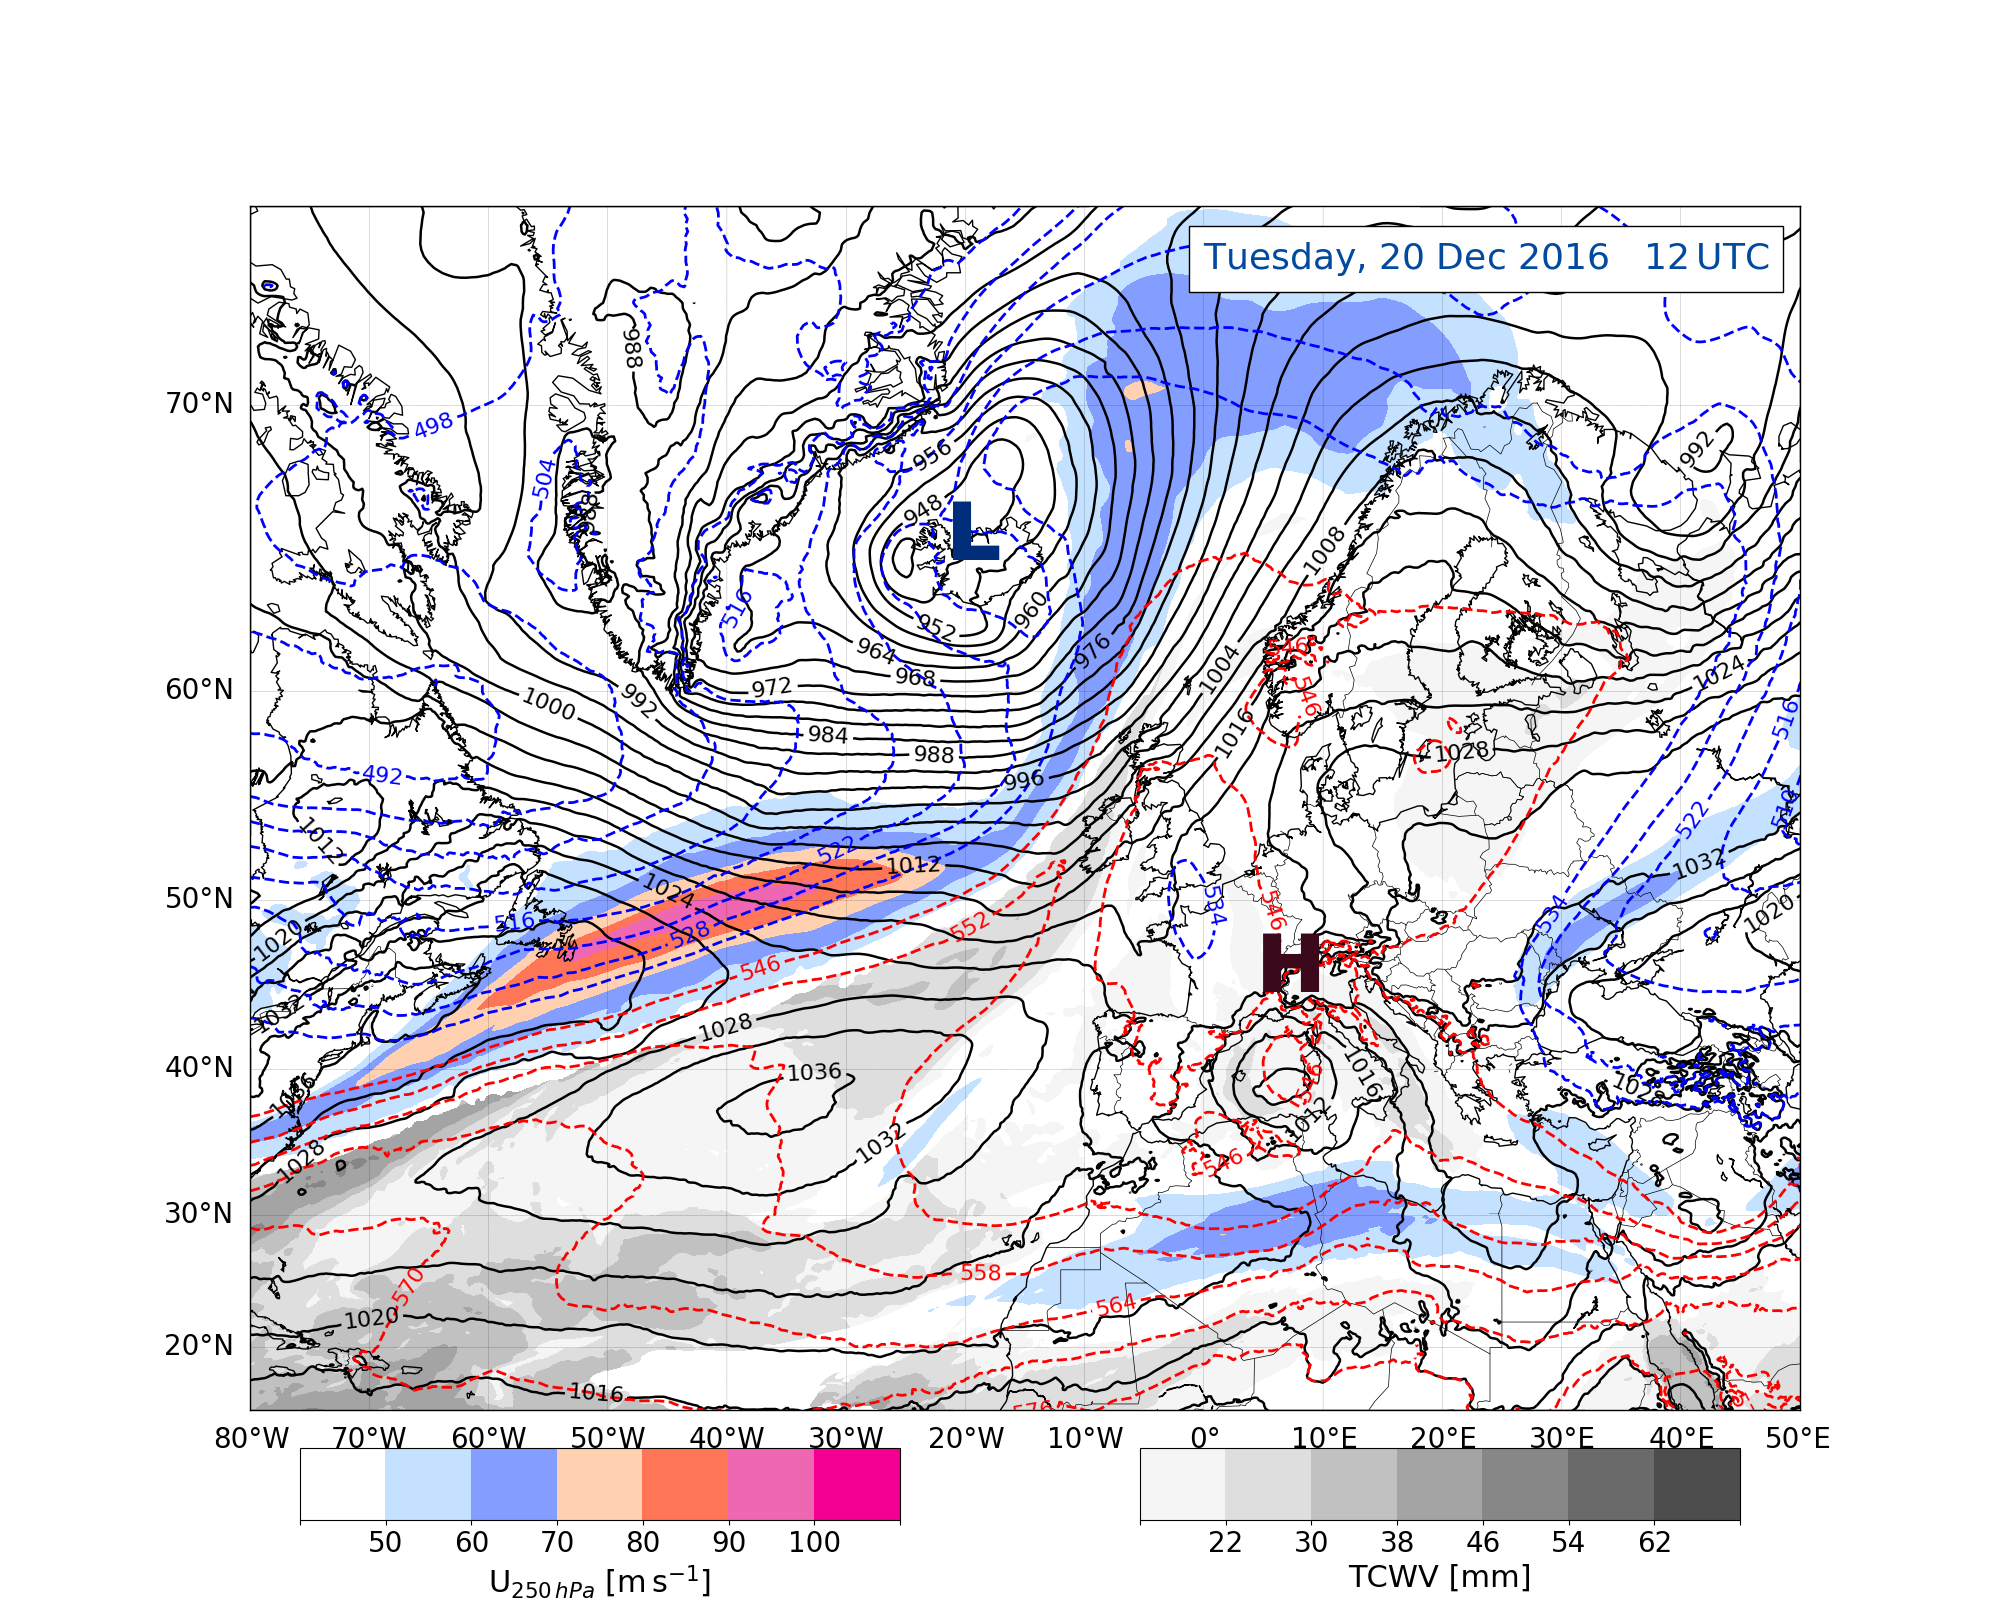
\includegraphics[trim={4.2cm 3.9cm 4.3cm 5.1cm},clip,
        width=\textwidth]{./fig_Geopot_Jet/20161220_12}
        \caption{}\label{fig:GP20}
        %\label{fig:DT2100}
    \end{subfigure}
%%%%%% 21/12
    \begin{subfigure}[b]{0.49\textwidth}
        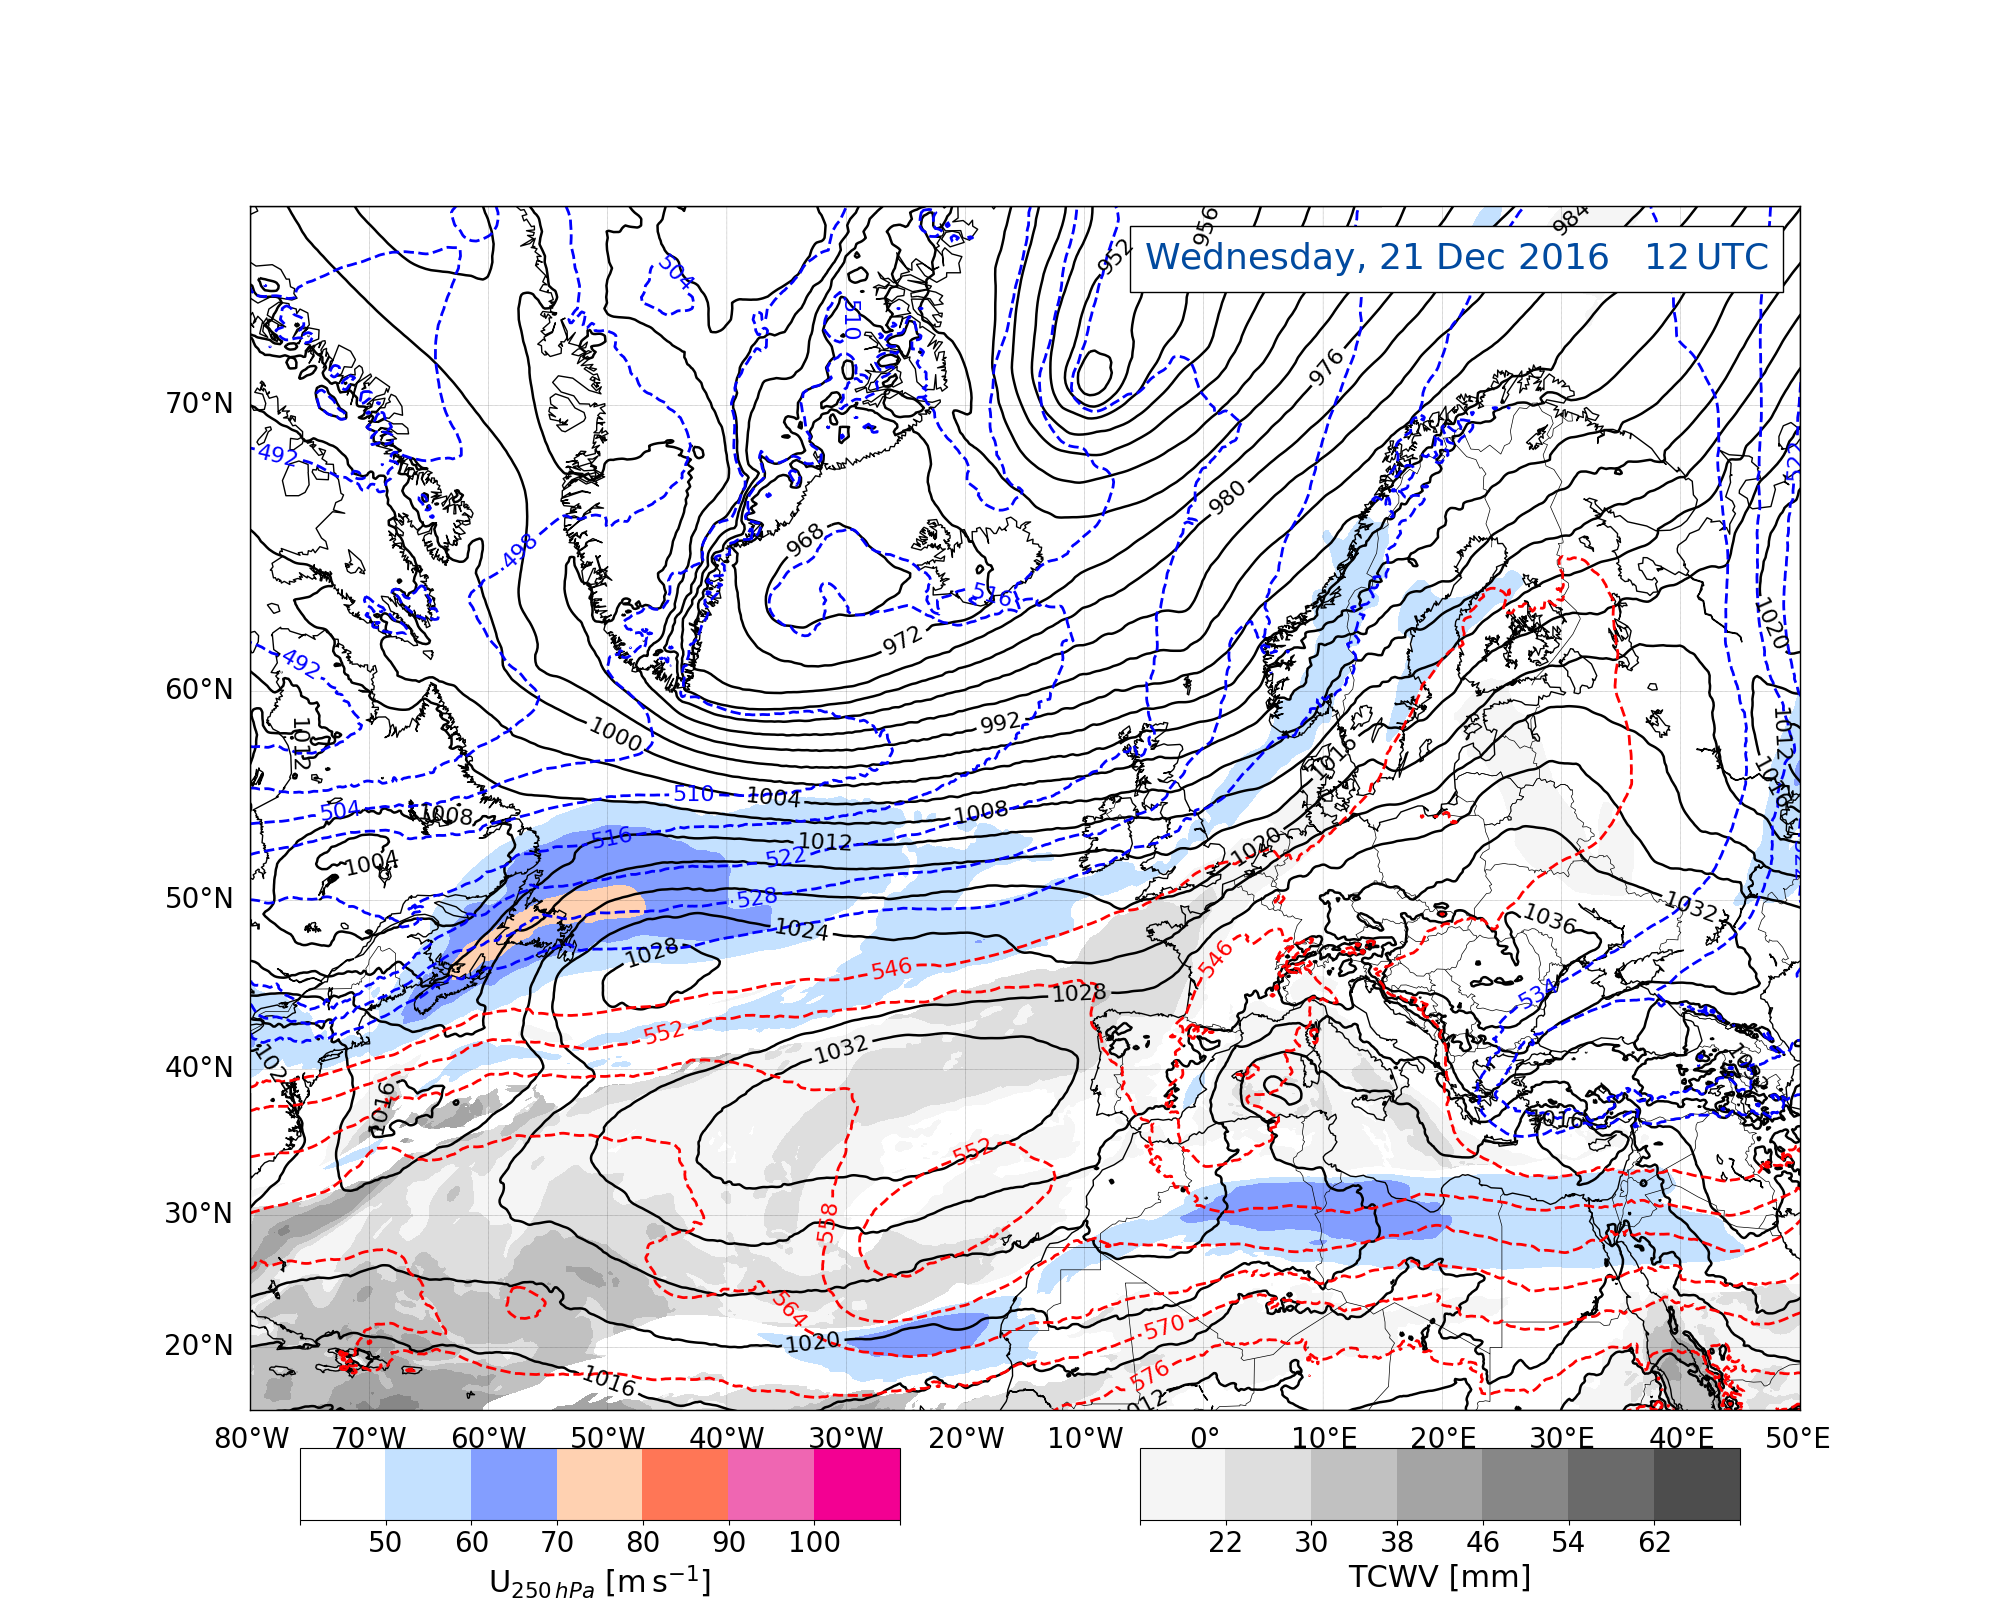
\includegraphics[trim={4.2cm 3.9cm 4.3cm 5.1cm},clip,
        width=\textwidth]{./fig_Geopot_Jet/20161221_12}
        \caption{}\label{fig:GP21}
    \end{subfigure}
%%%%%% 22/12
	\begin{subfigure}[b]{0.49\textwidth}
		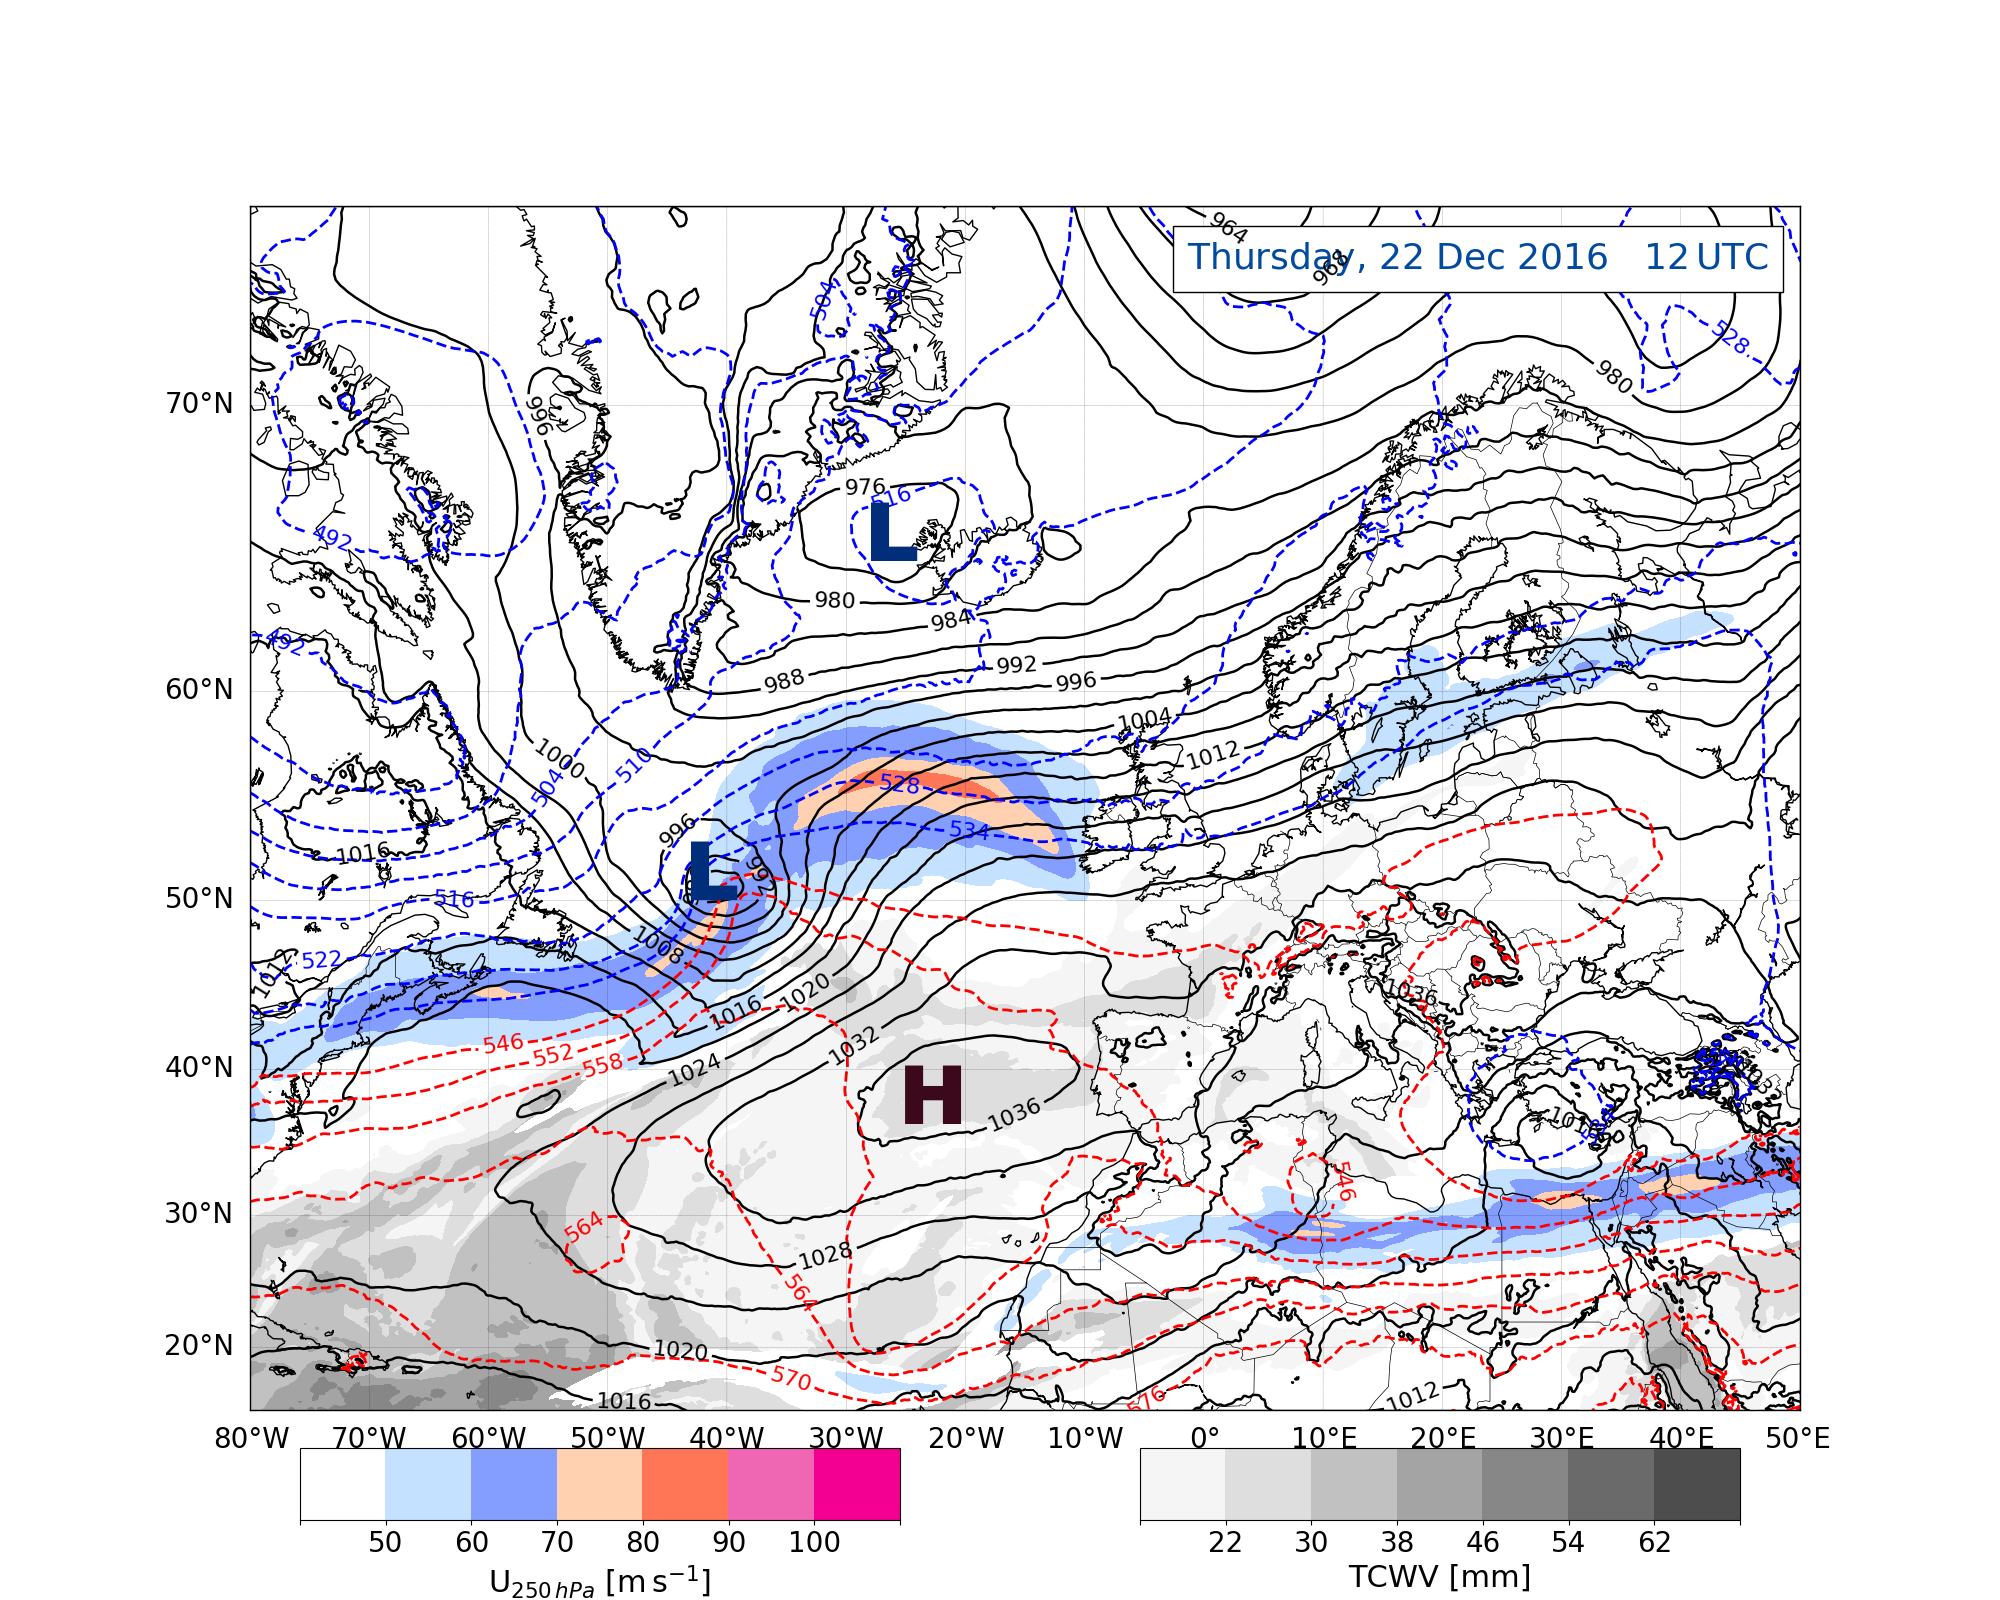
\includegraphics[trim={4.2cm 3.9cm 4.3cm 5.1cm},clip,
	width=\textwidth]{./fig_Geopot_Jet/20161222_12}
		\caption{}\label{fig:GP22}
	%\label{fig:sfc2100}
	\end{subfigure}
%%%%%% 23/12
	\begin{subfigure}[b]{0.49\textwidth}
		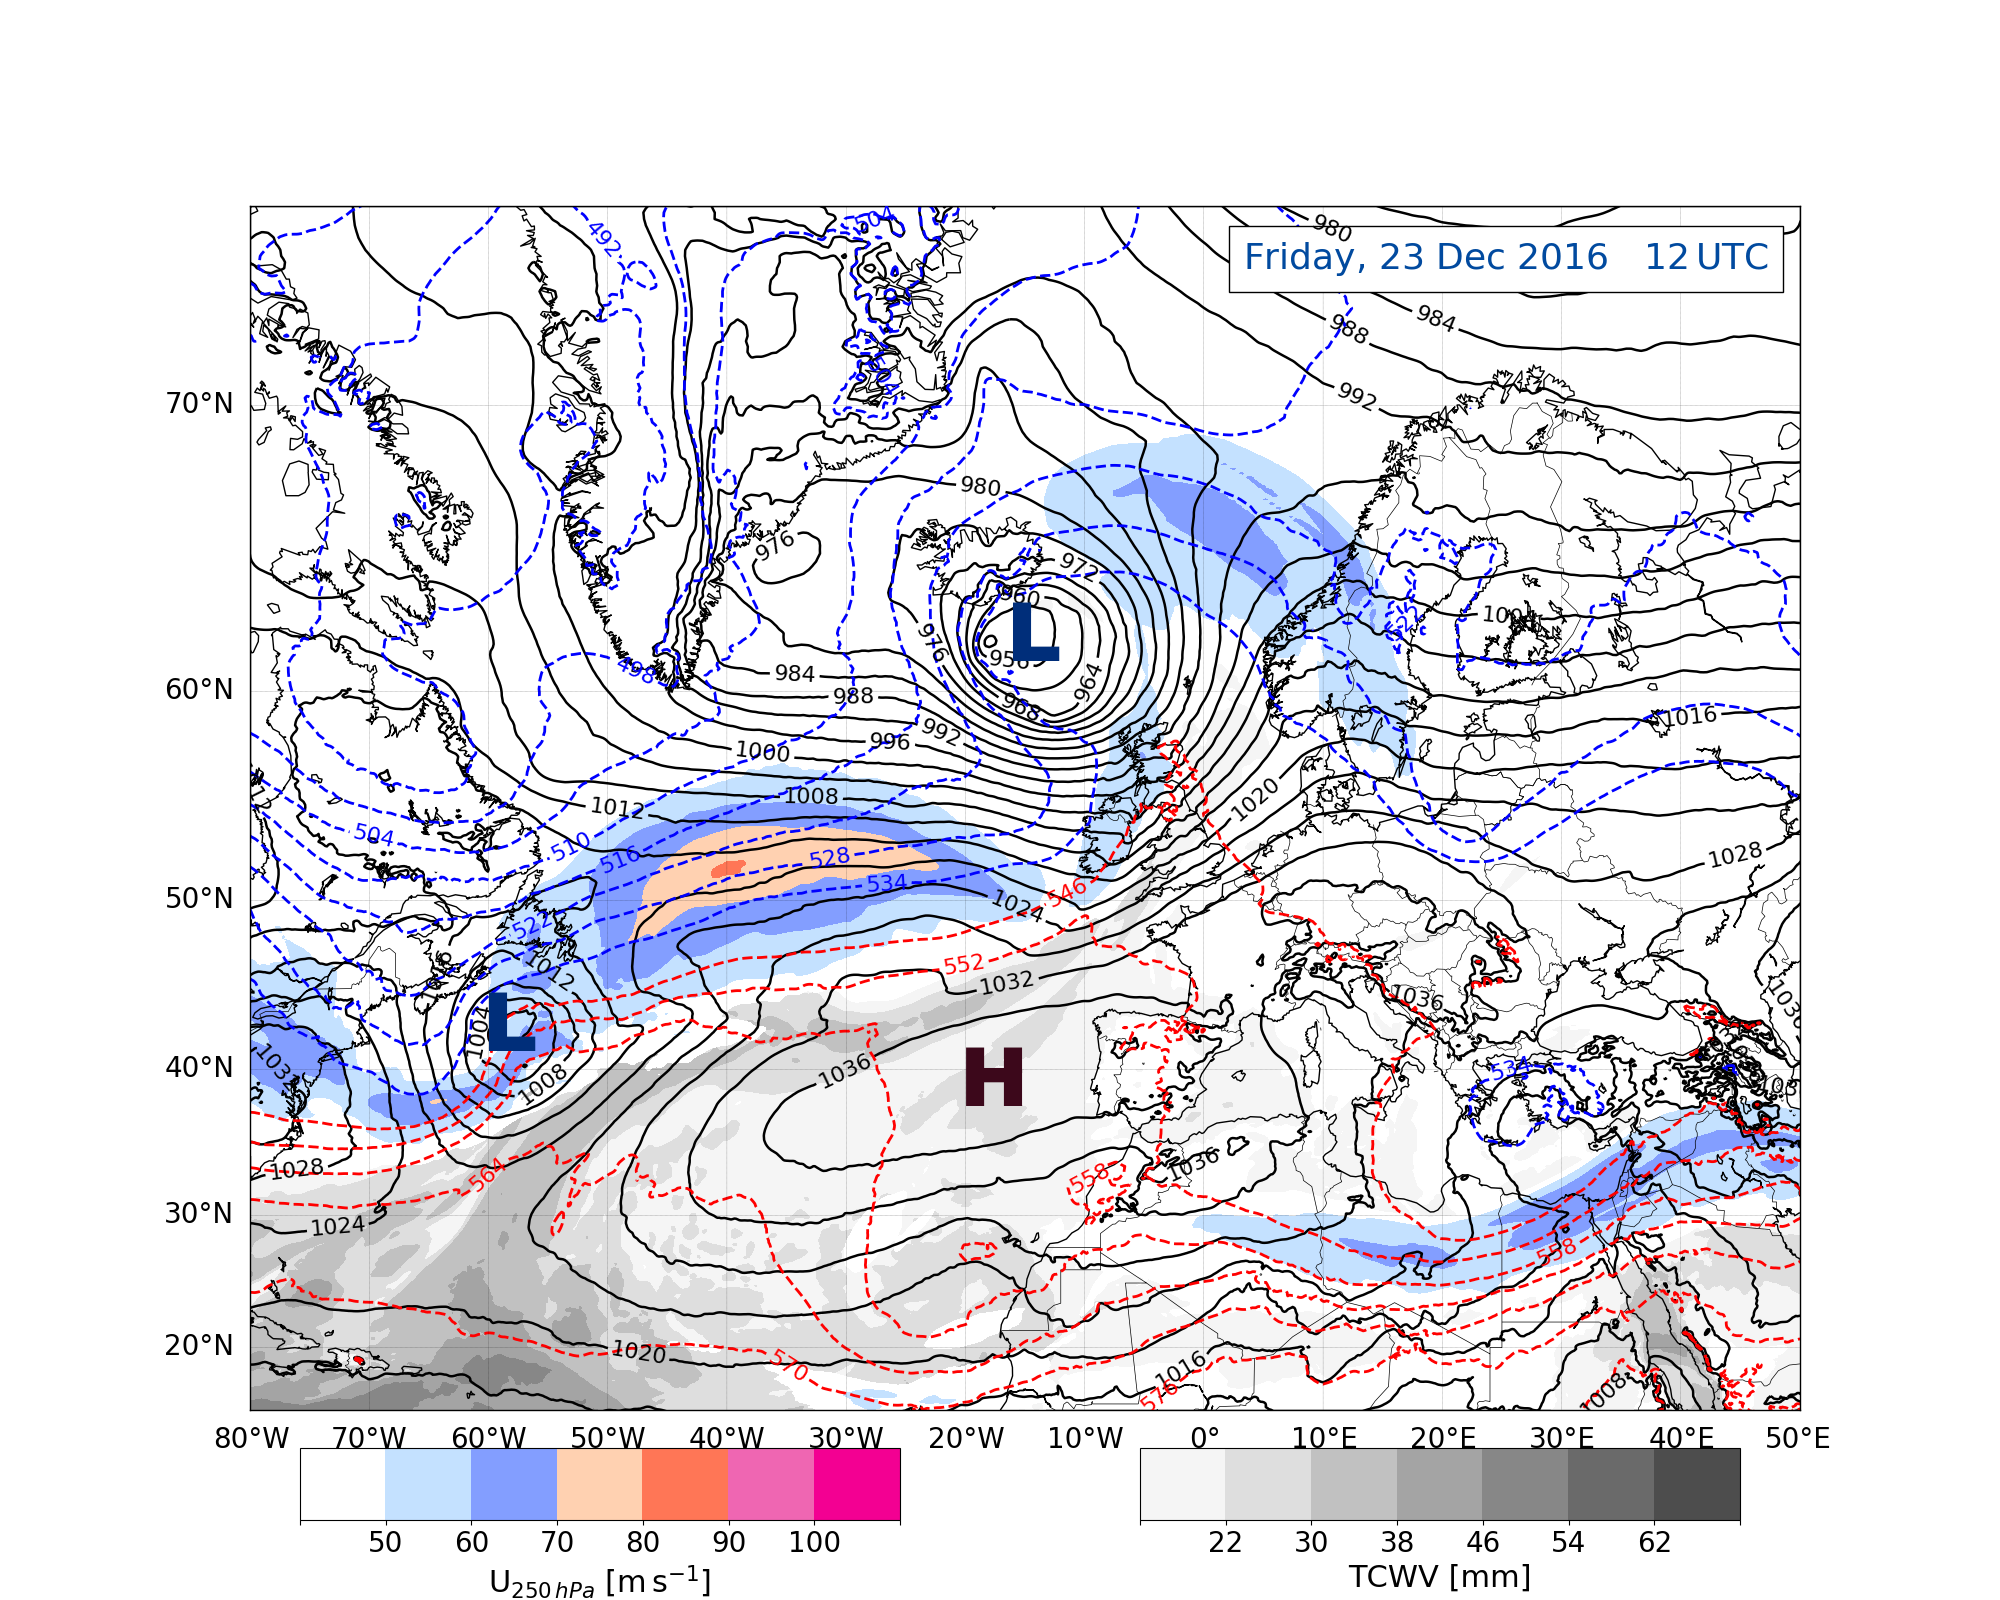
\includegraphics[trim={4.2cm 3.9cm 4.3cm 5.1cm},clip,
	width=\textwidth]{./fig_Geopot_Jet/20161223_12}
		\caption{}\label{fig:GP23}
	\end{subfigure}
%%%%%% label
    \begin{subfigure}[b]{\textwidth}
        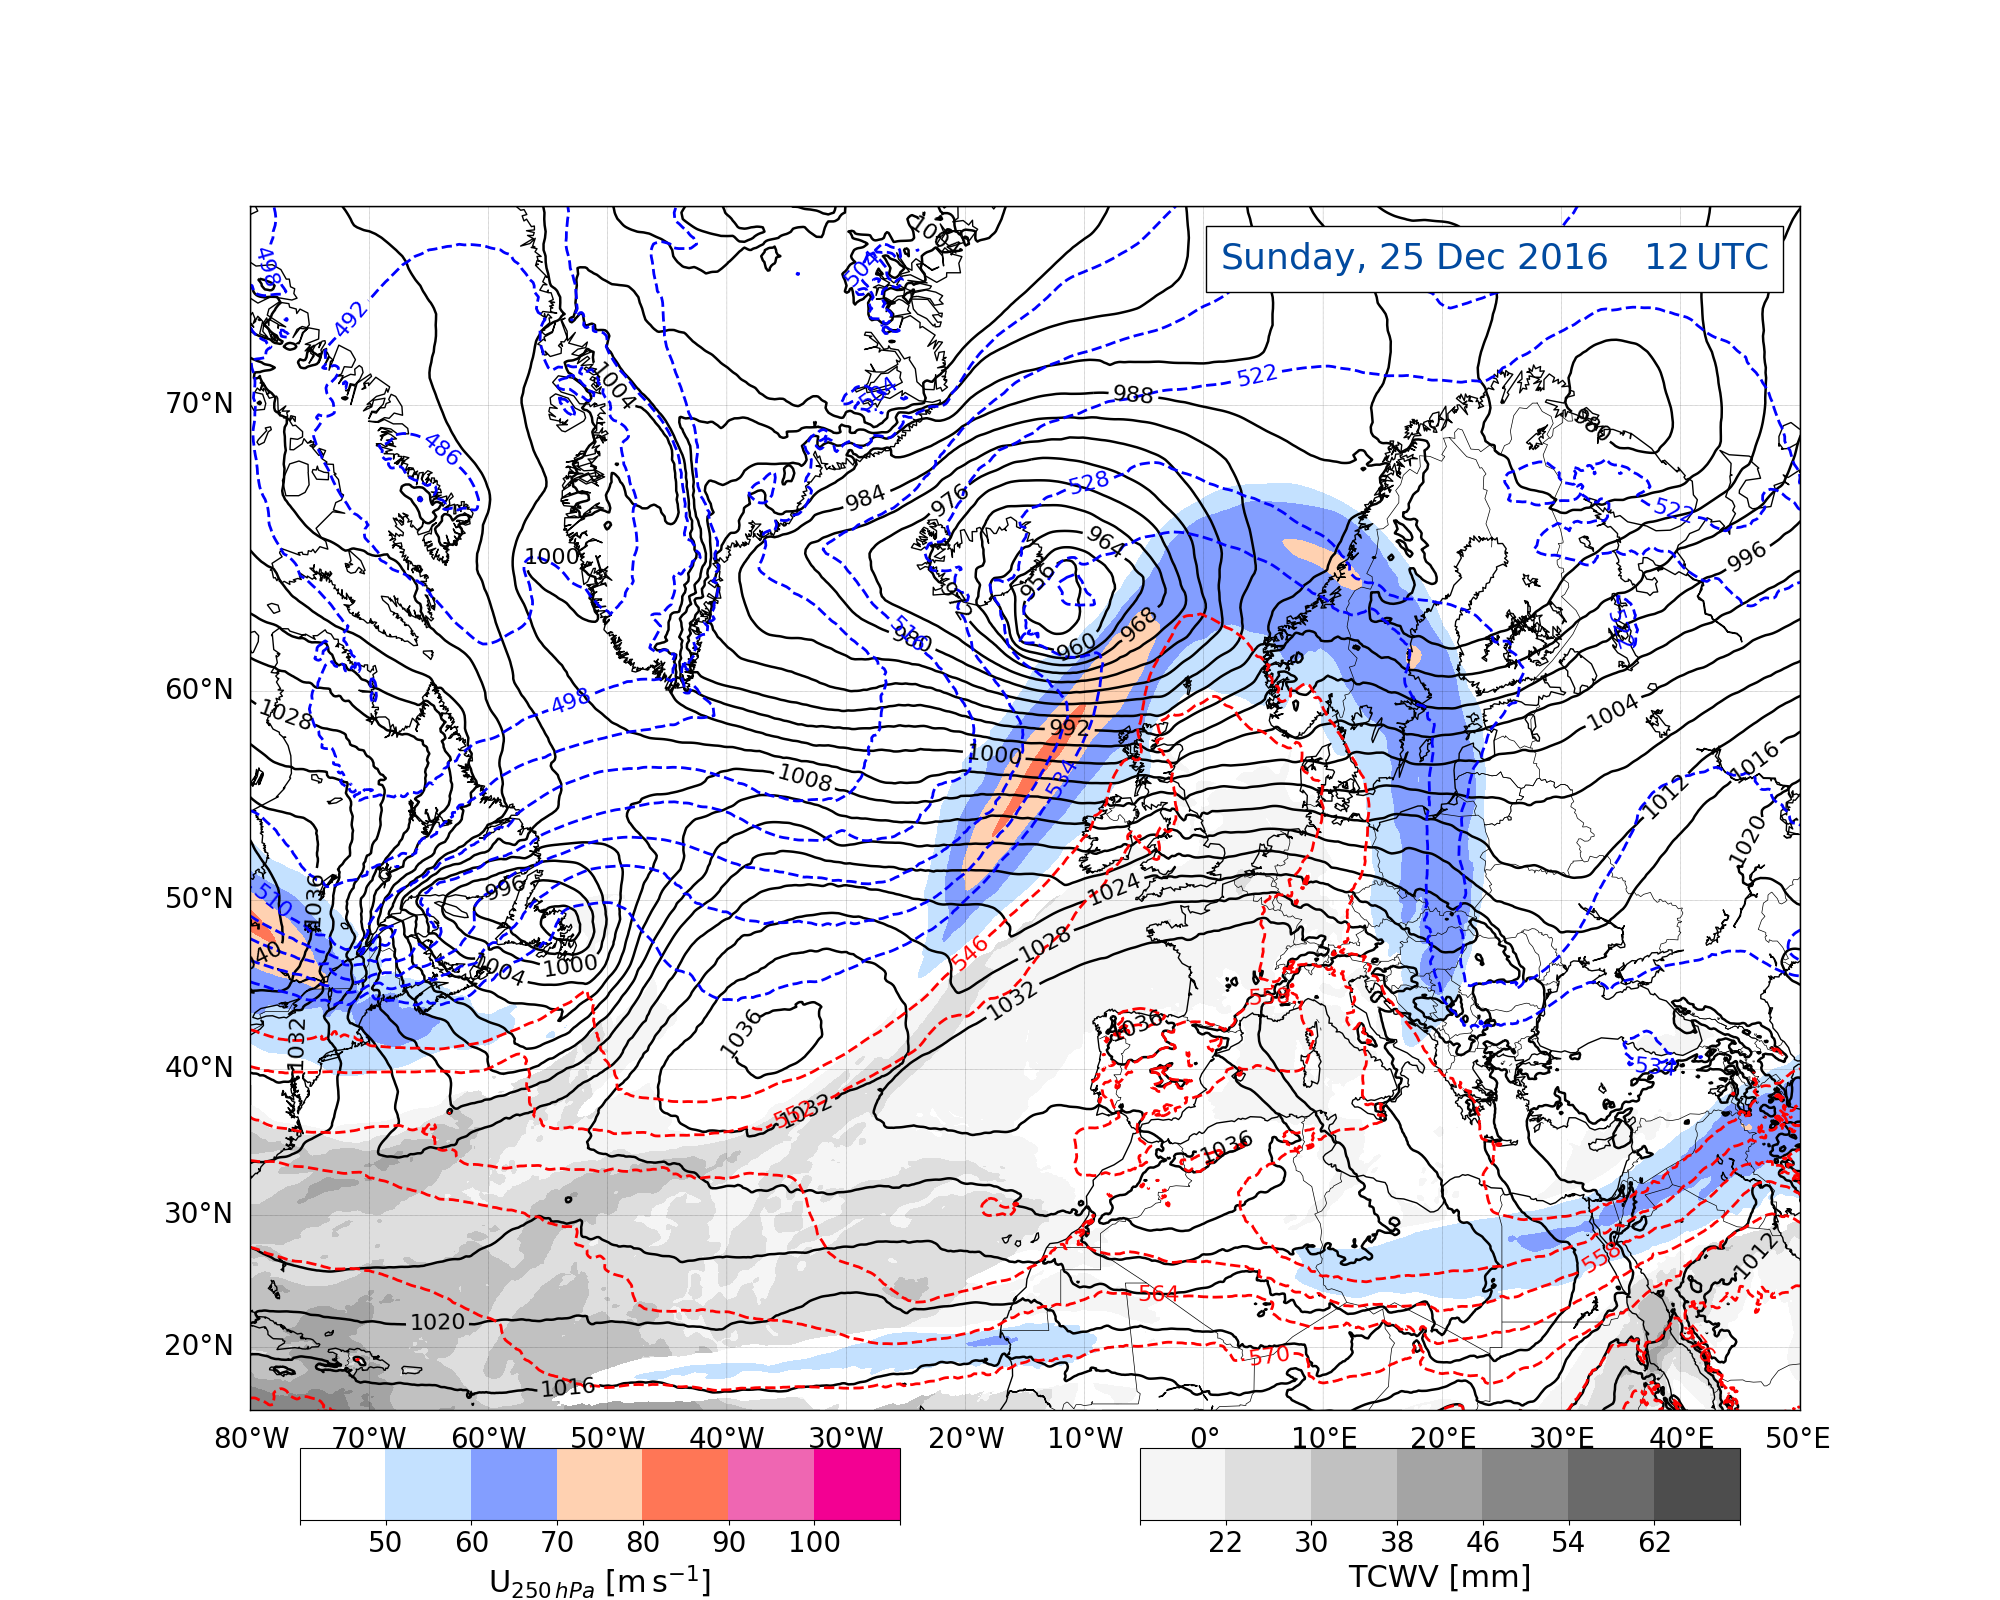
\includegraphics[trim={4.2cm 0cm 4.3cm 36.8cm},clip,
        width=\textwidth]{./fig_Geopot_Jet/20161225_12}
    \end{subfigure}
\caption{Jet, thickness, mean sea level pressure, and moisture synoptic analysis, data from ECMWF. During \SIrange{20}{27}{\dec}. \SI{250}{\hPa} wind speed, shaded according to the colour bar, [\SI{}{\mPs}]. \SI{1000}-\SI{500}{\hPa} thickness, dashed contours every \SI{6}{\deca\meter}, MSLP, black contours every \SI{4}{\hPa}, total column water vapour [\SI{}{\mm}], shaded according the grey scale.}\label{fig:GeopJet}
\end{figure}
\begin{figure}\ContinuedFloat
	\centering
%%%%%% 24/12
    \begin{subfigure}[b]{0.49\textwidth}
        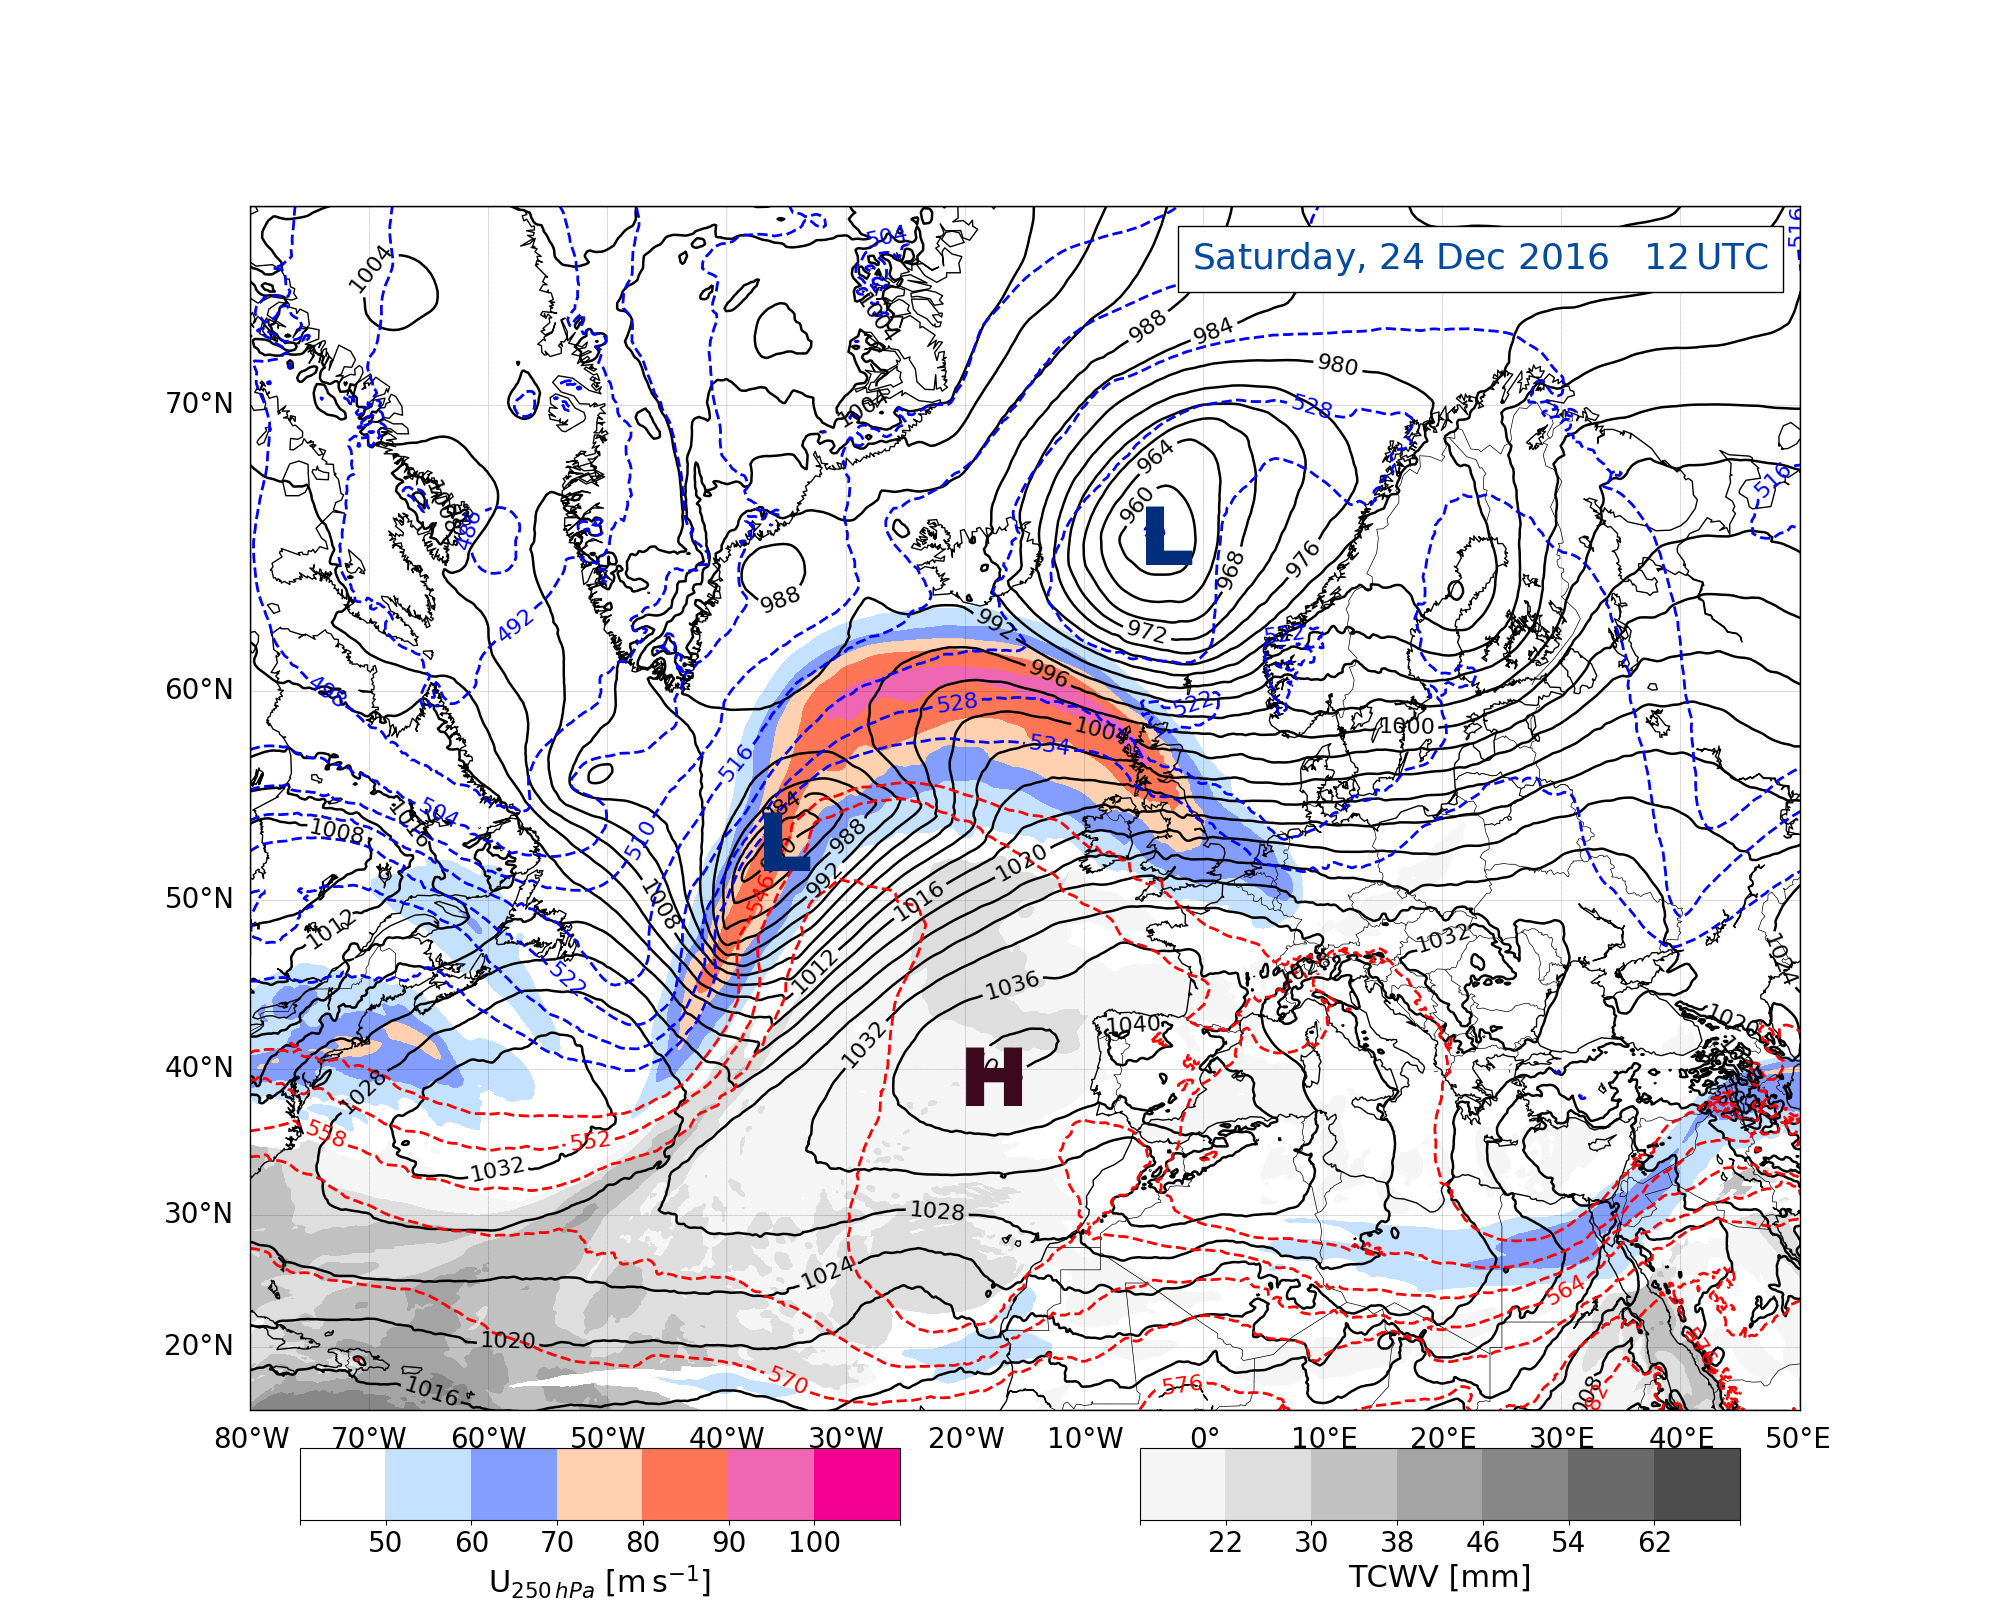
\includegraphics[trim={4.2cm 3.9cm 4.3cm 5.1cm},clip,
        width=\textwidth]{./fig_Geopot_Jet/20161224_12}
        \caption{}\label{fig:GP24}
    \end{subfigure}
%%%%%% 25/12
    \begin{subfigure}[b]{0.49\textwidth}
        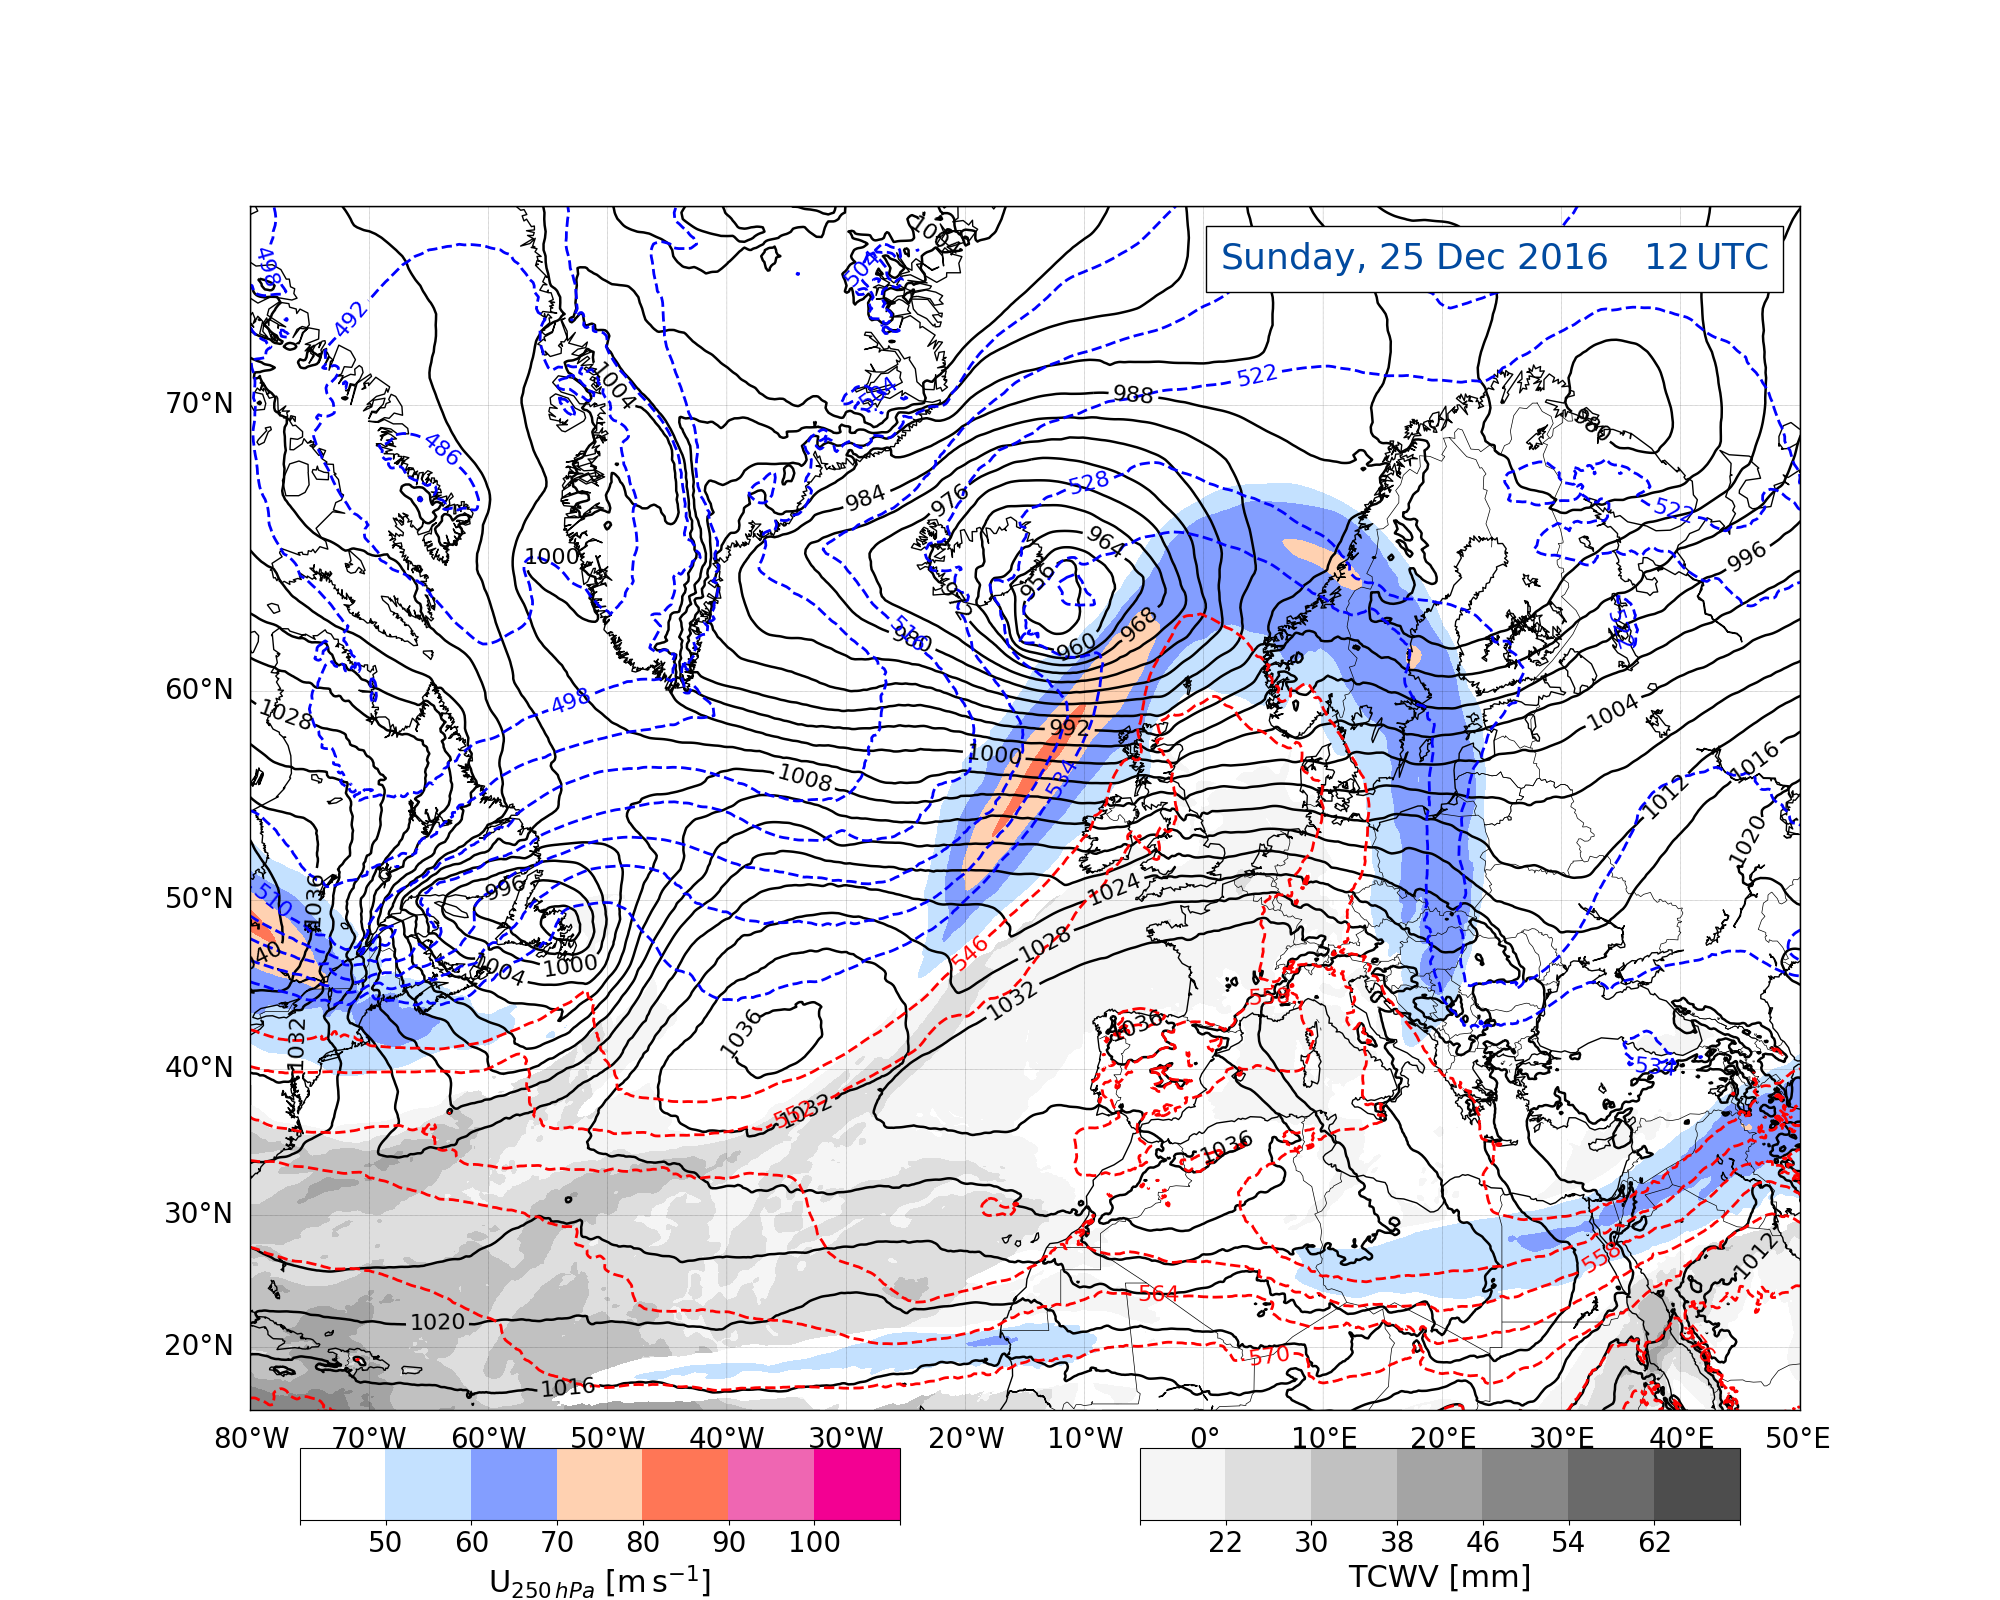
\includegraphics[trim={4.2cm 3.9cm 4.3cm 5.1cm},clip,
        width=\textwidth]{./fig_Geopot_Jet/20161225_12}
        \caption{}\label{fig:GP25}
    \end{subfigure}
%	\centering
%%%%%% 26/12
    \begin{subfigure}[b]{0.49\textwidth}
        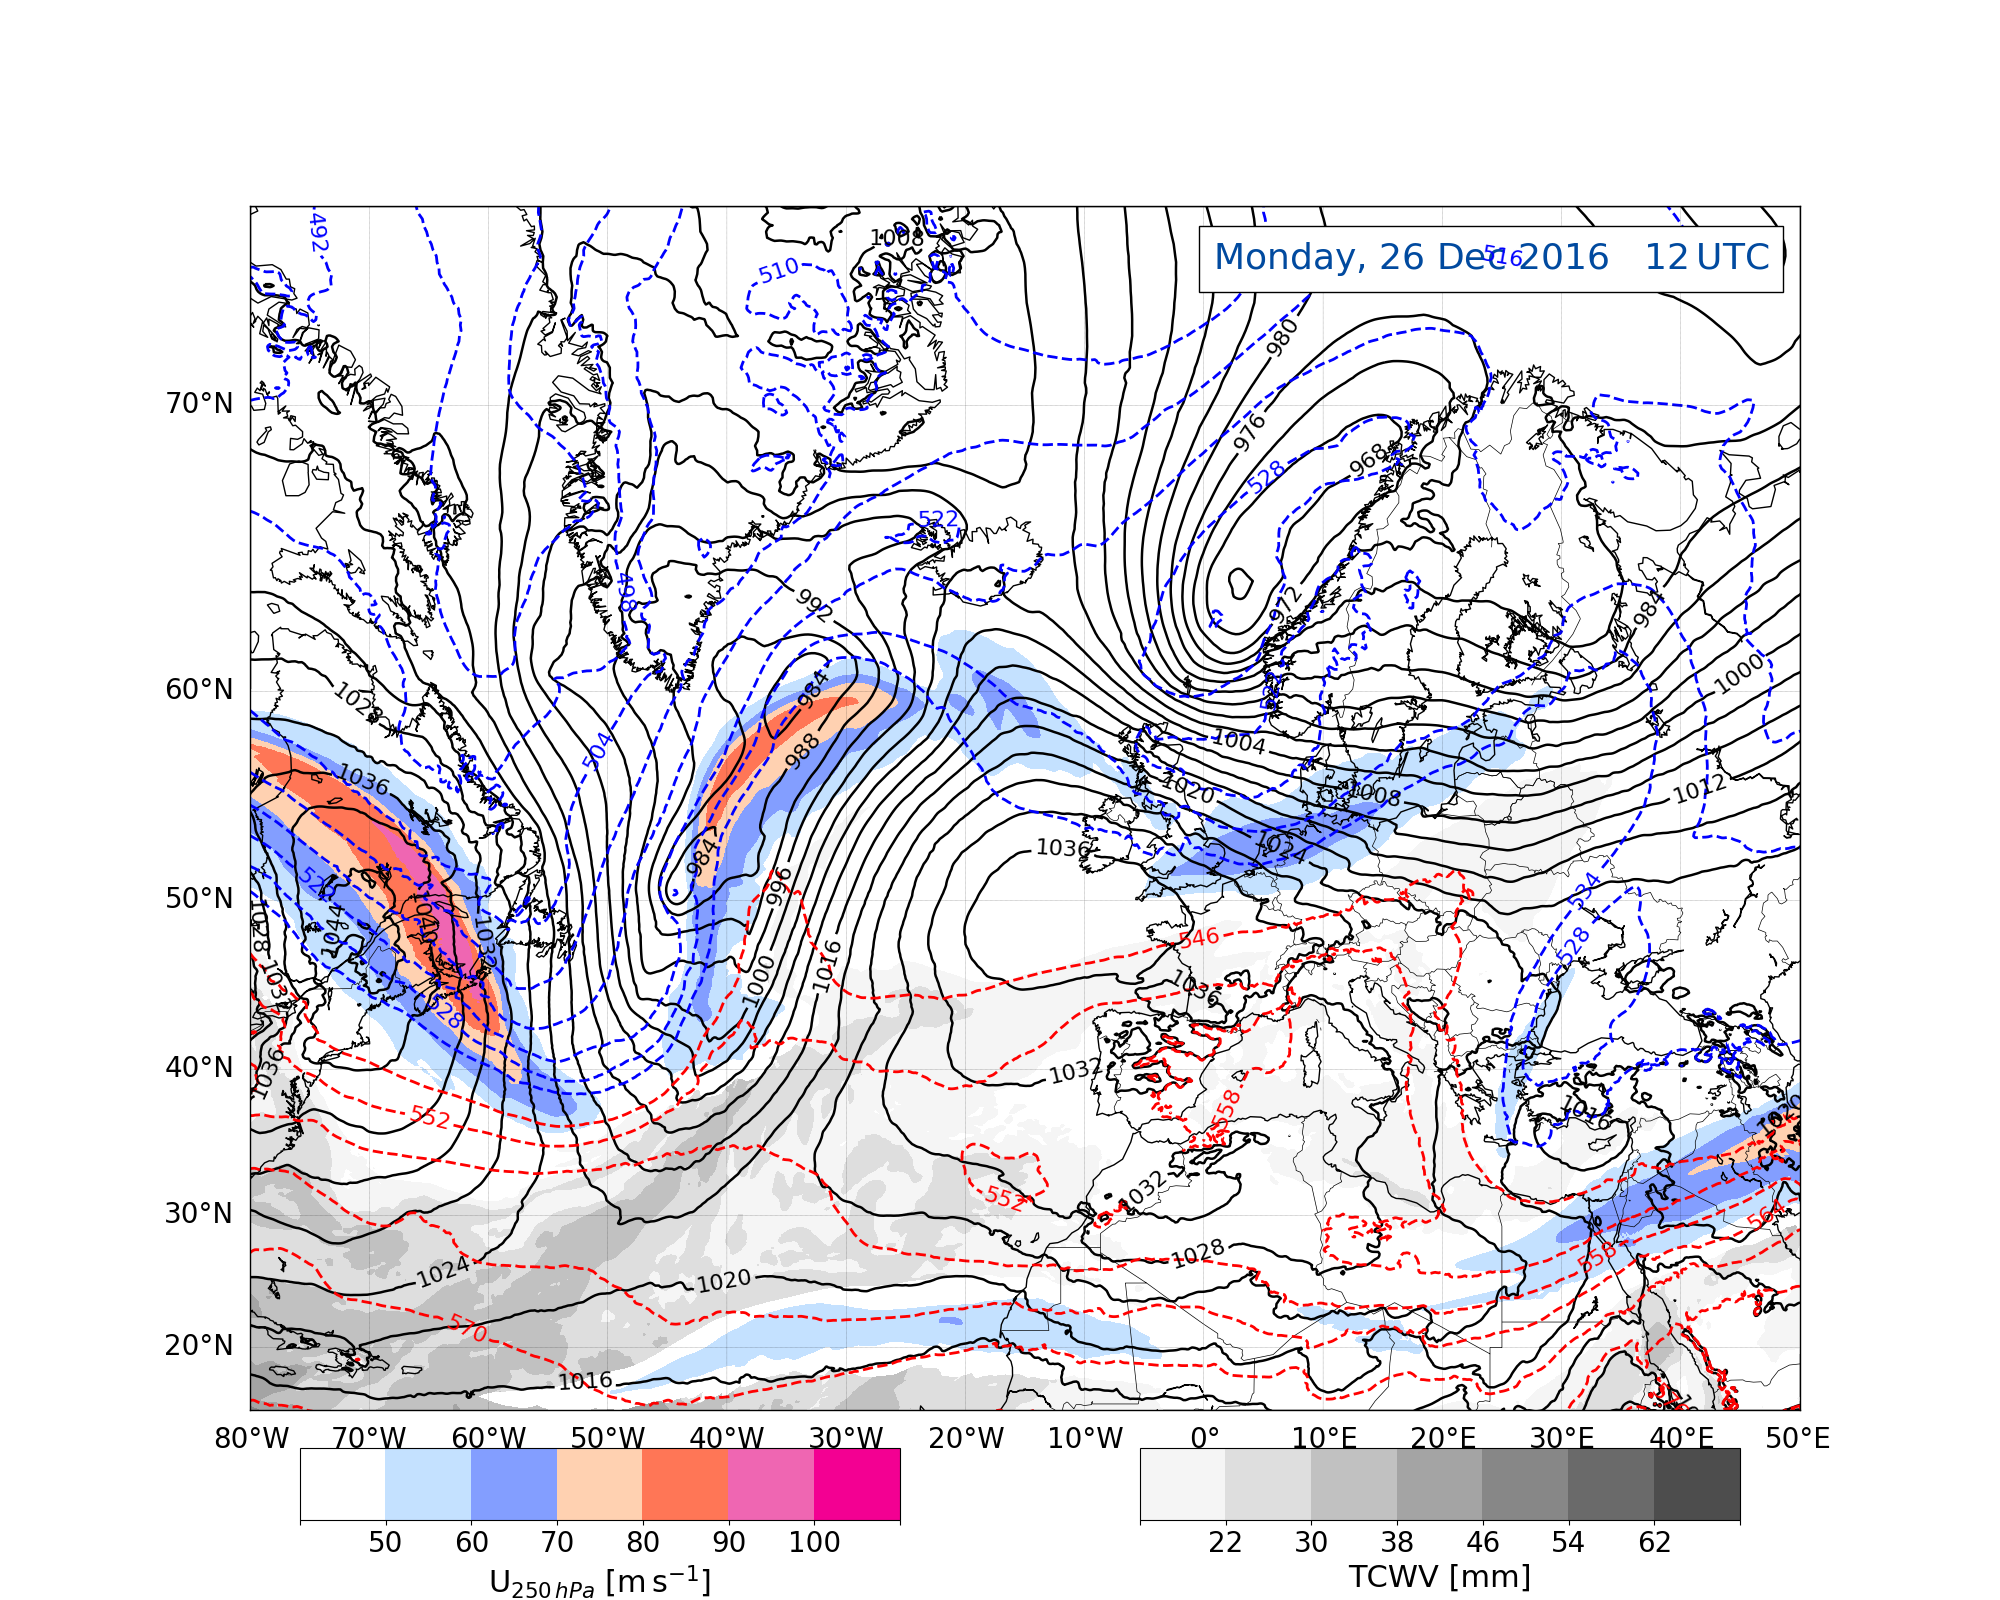
\includegraphics[trim={4.2cm 3.9cm 4.3cm 5.1cm},clip,
        width=\textwidth]{./fig_Geopot_Jet/20161226_12}
        \caption{}\label{fig:GP26}
    \end{subfigure}
%%%%%% 27/12
    \begin{subfigure}[b]{0.49\textwidth}
        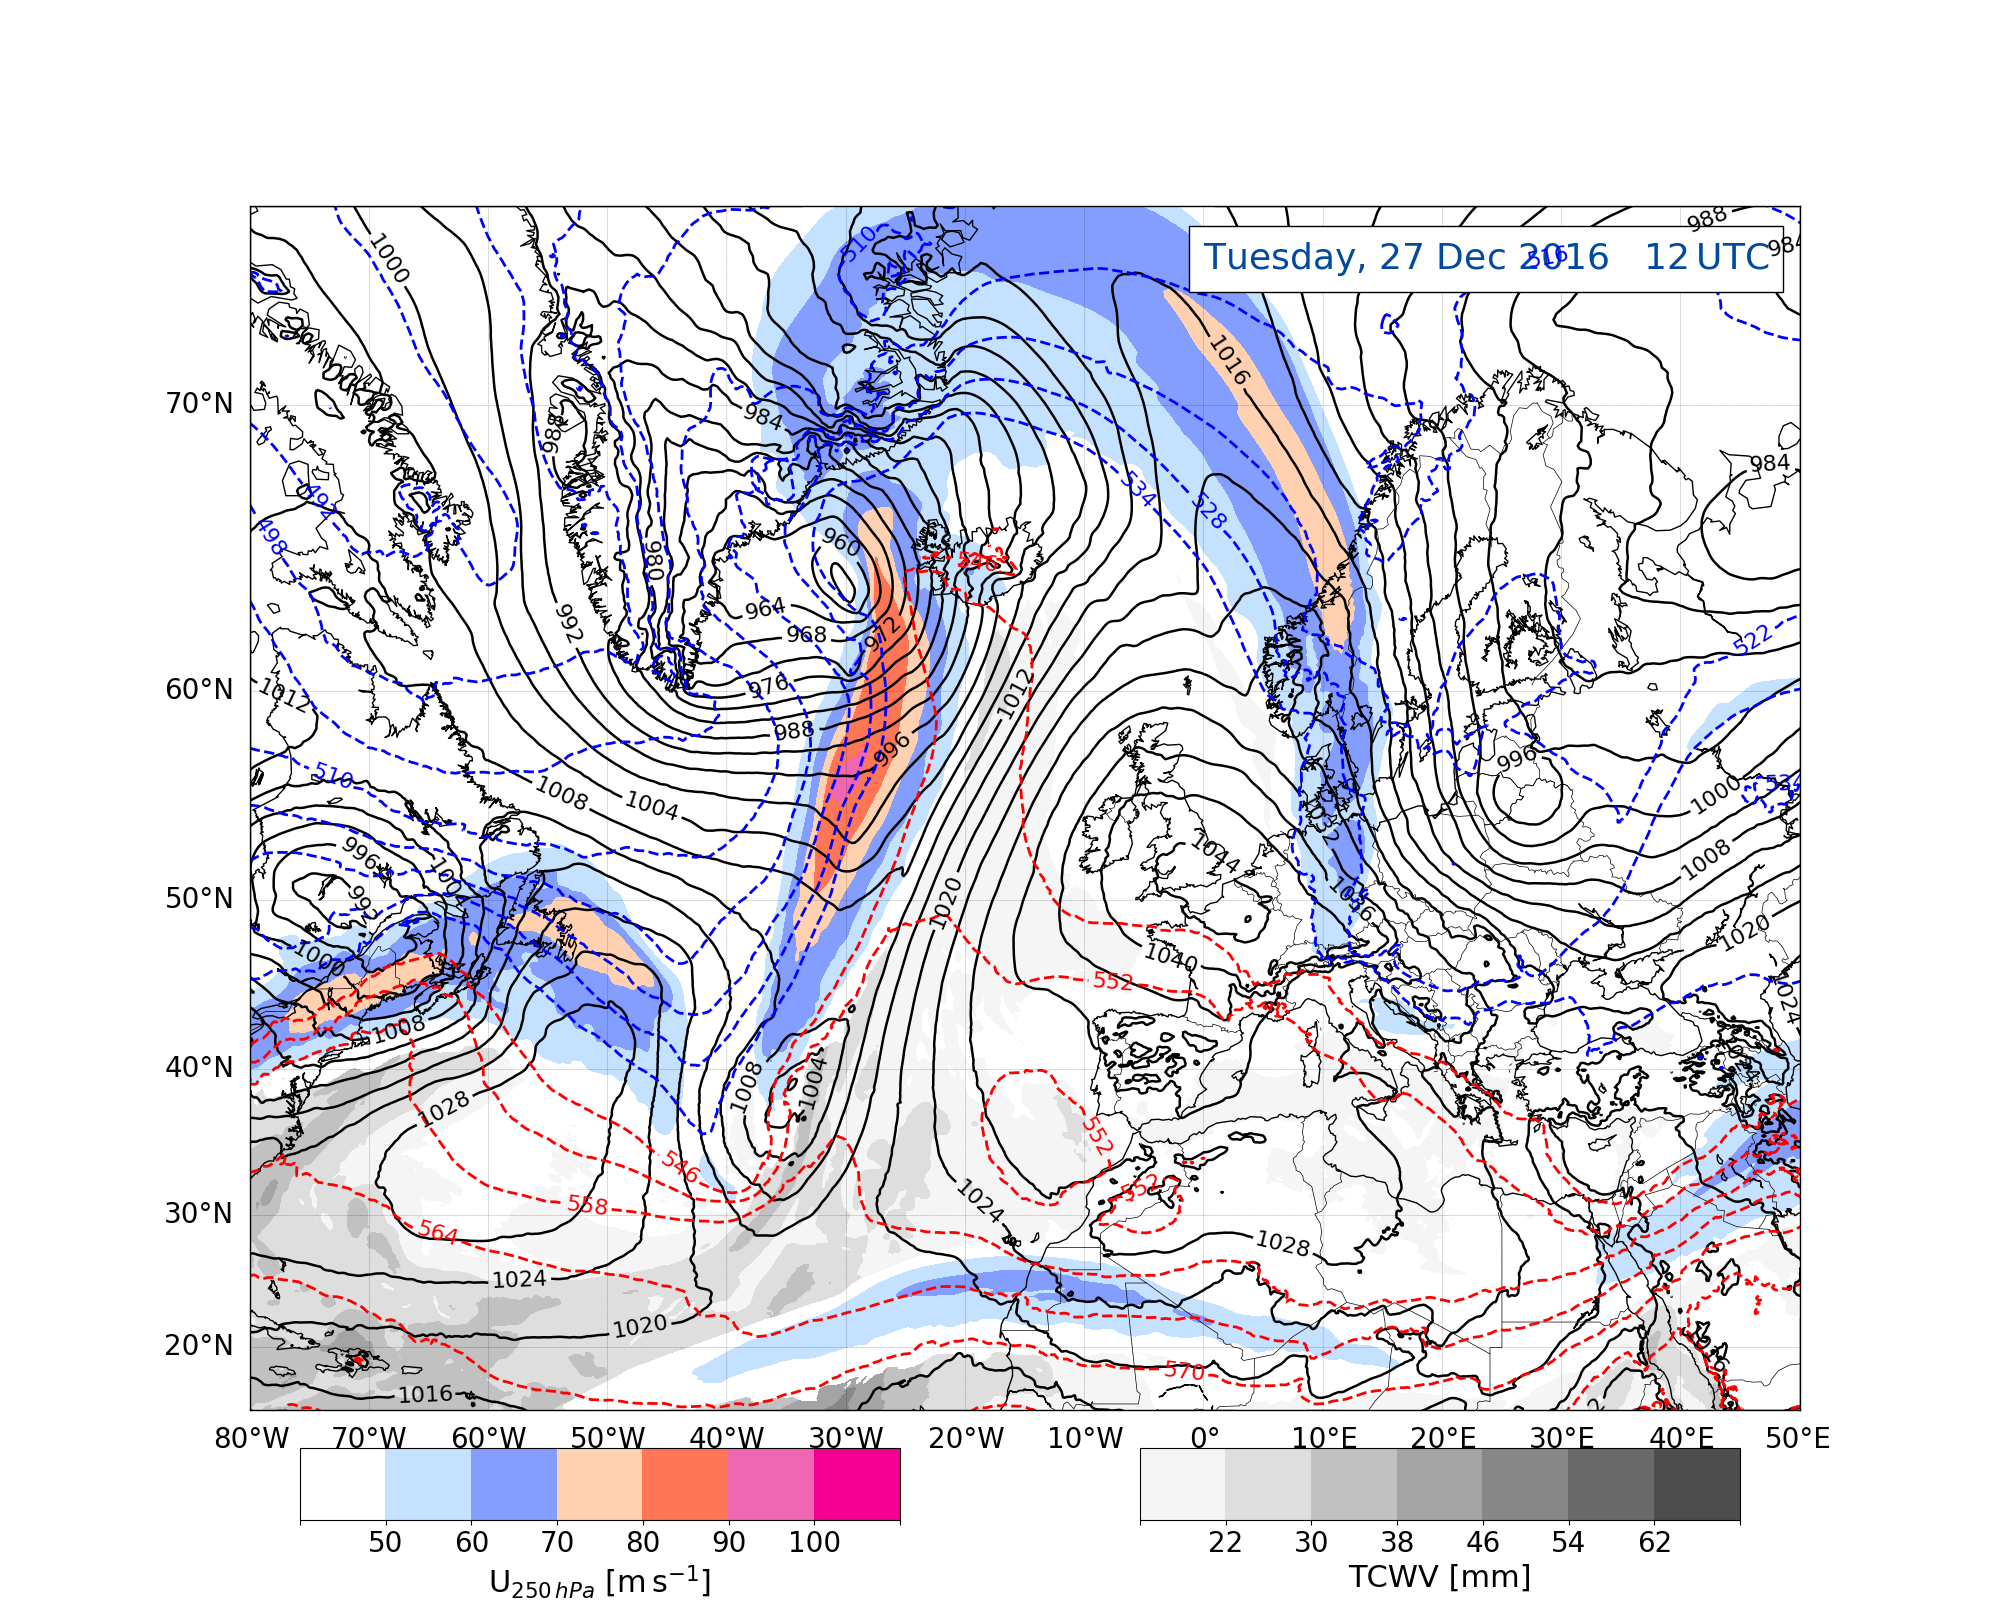
\includegraphics[trim={4.2cm 3.9cm 4.3cm 5.1cm},clip,
        width=\textwidth]{./fig_Geopot_Jet/20161227_12}
        \caption{}\label{fig:GP27}
    \end{subfigure}
%%%%%% label
    \begin{subfigure}[b]{\textwidth}
        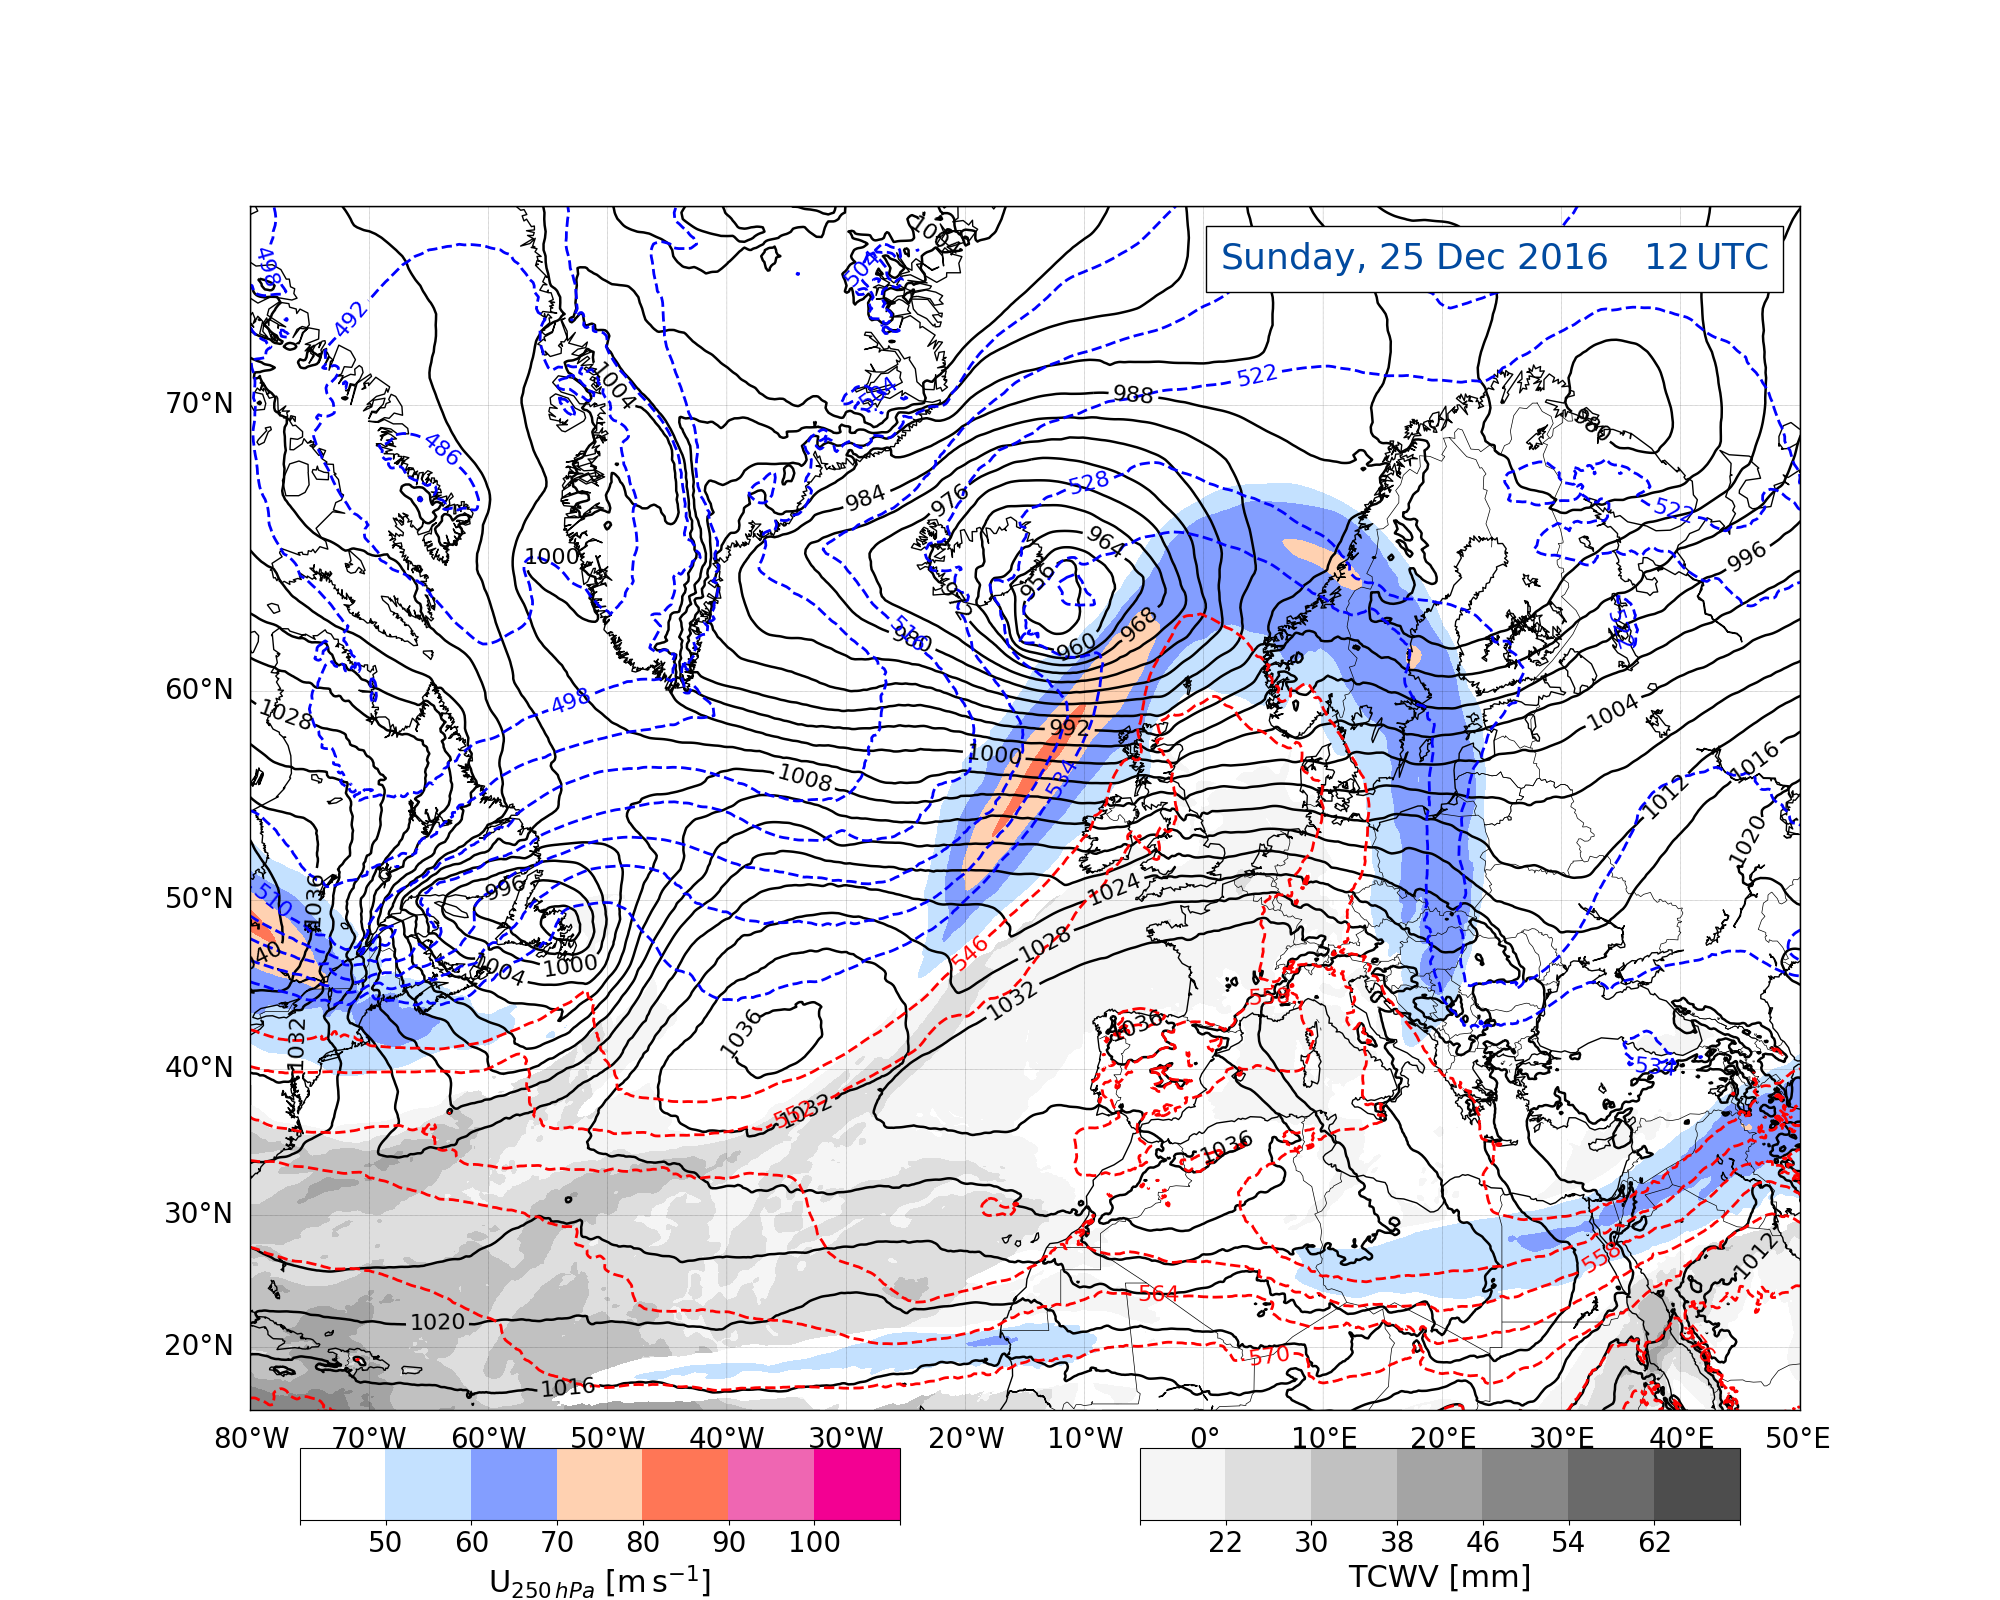
\includegraphics[trim={4.2cm 0cm 4.3cm 36.8cm},clip,
        width=\textwidth]{./fig_Geopot_Jet/20161225_12}
       % \label{fig:D}
    \end{subfigure}
\caption{\textit{(Continued from previous page.)}}   
\end{figure}
%%%%%%%%%%%%%%%%%%%%%%%%%%%%%%%%%%%%%%%%%%%%%%%%%%%%%%%%%%%%%%%%%%%%%%%%%%